\chapter{التطبيق خطوة بخطوة من الصفر}
\label{ch:01b-build}

\section{قبل أن تبدأ}
\label{sec:build-start}

يبني هذا الفصل السيناريو كله في مؤسستك بالترتيب، من الوحدات التنظيمية حتى قرار المدقق، ثم لوحة مؤشرات للمنشآت الصناعية. نُفّذت كل خطوة فيه فعلاً وجُرّب كل قرار، والصور من ذلك التنفيذ. اتبع الترتيب كما هو؛ فكل خطوة تحتاج إلى ما أُنشئ قبلها.

تحتاج إلى حساب مسؤول يستطيع فتح «ادوات البناء» و«الإعدادات». وإذا كان لدى مؤسستك بيئة تجريبية، فابدأ بها قبل البيئة الفعلية.

\begin{rcnote}[مثال: مديرية الواحة]
تستخدم الخطوات الأسماء والرموز في الجدول التالي. استبدلها بأسماء جهتك، واحتفظ بالرموز القصيرة لأنها تظهر بجانب كل اسم في القوائم.
\end{rcnote}

\begin{table}[H]
\centering
\caption{ما الذي ستنشئه؟}
\label{tab:build-plan}
\begin{tabularx}{\linewidth}{R{3.4cm} Y}
\rcHeaderRow
\thh{السجل} & \thh{مثال الواحة}\\
وحدتان تنظيميتان & مديرية الواحة لحماية المستهلك \en{(WAHA)}، وتحتها دائرة الرقابة الميدانية \en{(WAHA-FLD)}.\\
ثلاثة أوصاف وظيفية & باحث ميداني، ومدقق كشوف، ورئيس فريق الكشف.\\
ثلاثة مناصب & رئيس فريق الكشف، وباحث ميداني أول، ومدقق كشوف.\\
ثلاثة أعضاء & خالد العلي، وليلى منصور، ورنا يوسف، ولكل منهم تعيين في منصبه.\\
مجموعتان وثلاثة أدوار & فريق الكشف ومدققو الكشوف؛ وأدوار للباحث والمدقق ورئيس الفريق.\\
تطبيق ونوع سجلات & تطبيق «حماية المستهلك - الواحة»، ونوع السجلات «منشآت الواحة»، وسجل «فرن السنابل».\\
نموذج وخطة & نموذج «كشف منشأة - الواحة» بمسار وموافقة، وخطة «جولة كشف الواحة».\\
\end{tabularx}
\end{table}

\section{أنشئ الوحدات التنظيمية}
\label{sec:build-nodes}

الوحدة التنظيمية مكان في هيكل الجهة، مثل مديرية أو دائرة. أنشئ الوحدة الأعلى أولاً، ثم الوحدات التي تتبعها.

\begin{rcnote}[مثال: مديرية الواحة]
تُنشأ «مديرية الواحة لحماية المستهلك» بالرمز \en{WAHA}، ثم «دائرة الرقابة الميدانية» بالرمز \en{WAHA-FLD}، وفي «يتبع ل» تُختار المديرية.
\end{rcnote}

\begin{figure}[H]
\centering
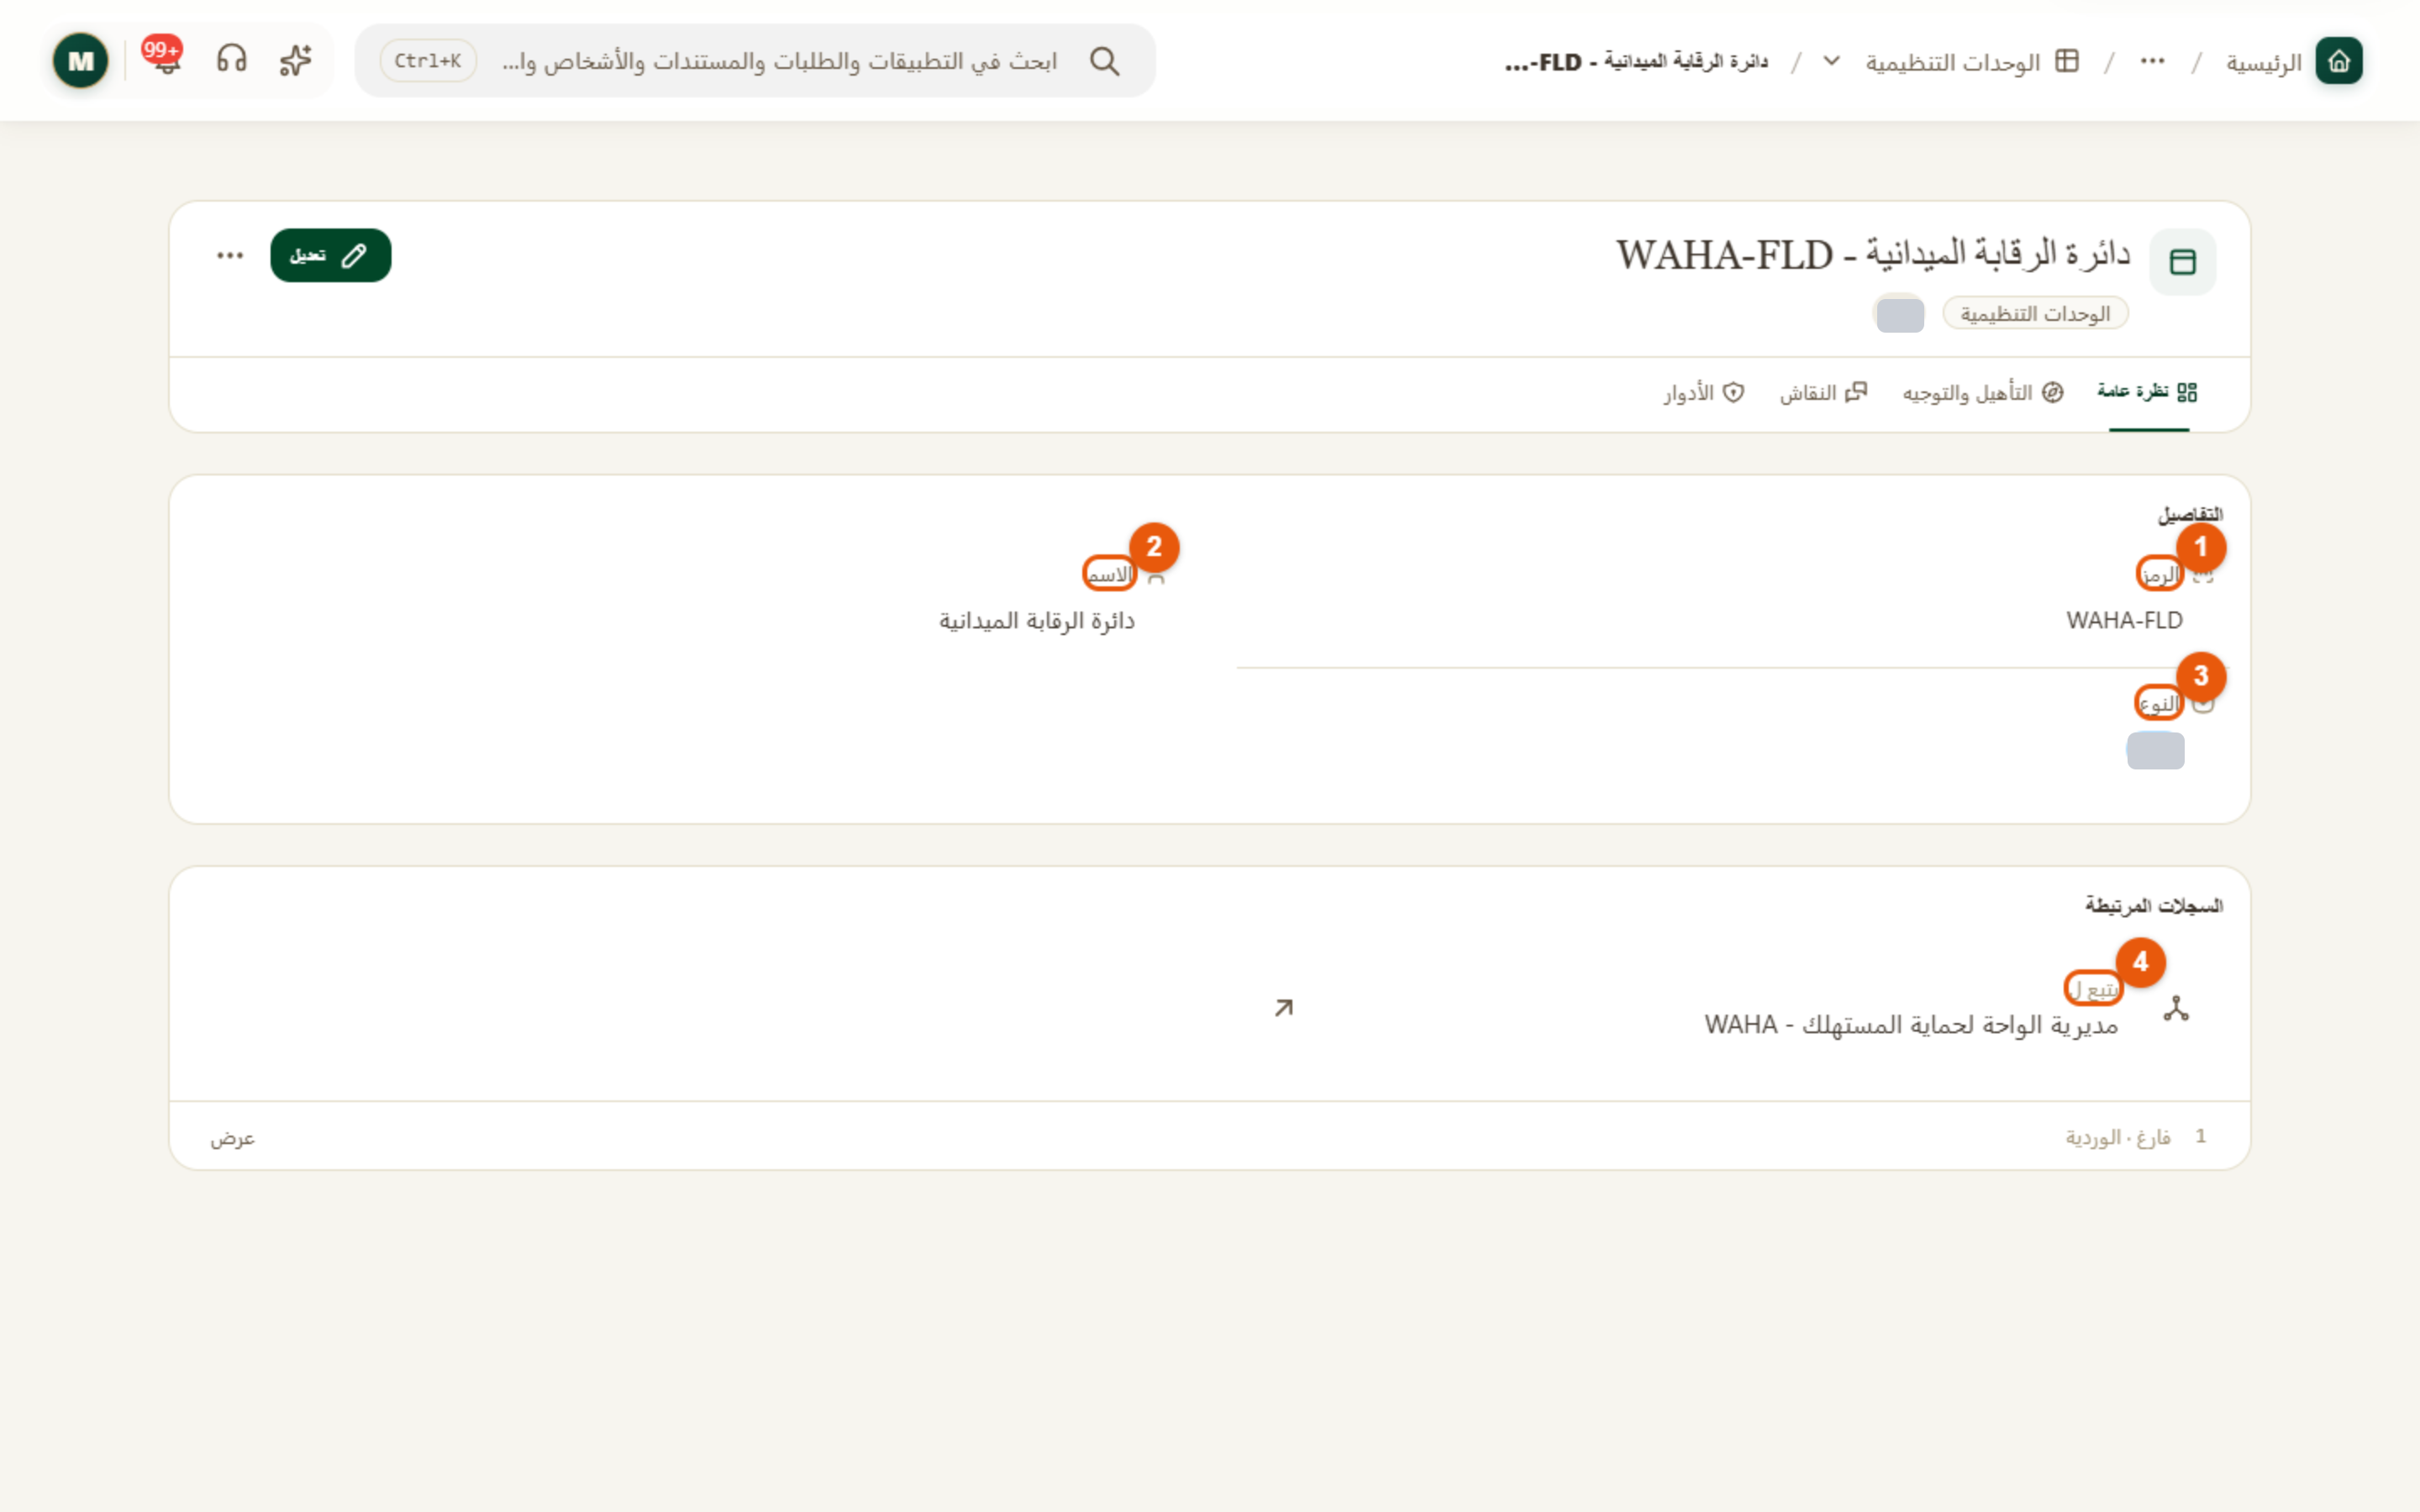
\includegraphics[width=0.95\linewidth]{assets/screens/b-node.png}
\caption{وحدة تنظيمية بعد إنشائها}
\label{fig:build-node}
\shotnote{يظهر اسم الوحدة في القوائم مع رمزها، مثل «دائرة الرقابة الميدانية - WAHA-FLD». وبهذا الشكل ستبحث عنها لاحقاً في كل حقل يرتبط بها. ① «الرمز»: قصير وفريد. ② «الاسم». ③ «النوع»: اختر من قائمة مؤسستك؛ فالقائمة تختلف من مؤسسة إلى أخرى، وقيمتها مخفية في الصورة. ④ «يتبع ل»: الوحدة الأعلى.}
\end{figure}

\subsection{خطوات العمل والتحقق}
\begin{enumerate}
\item افتح «الموارد البشرية» ← «الوحدات التنظيمية»، واضغط «سجل جديد».
\item اكتب «الرمز» و«الاسم»، واختر «النوع»، ثم اضغط «إنشاء».
\item أنشئ الوحدة الثانية بالطريقة نفسها، واختر في «يتبع ل» الوحدة الأولى. اكتب جزءاً من اسمها في مربع البحث، ثم اخترها من القائمة.
\end{enumerate}

\textbf{تحقق:} افتح الوحدة الثانية، ويجب أن تظهر الوحدة الأولى تحت «السجلات المرتبطة».

\section{أنشئ أوصاف الوظائف والمناصب}
\label{sec:build-positions}

يصف الوصف الوظيفي العمل، بينما يحدد المنصب مكانه في الوحدة ومن يرأسه. لذلك أنشئ الأوصاف أولاً، ثم المناصب التي تستخدمها.

\begin{rcnote}[مثال: مديرية الواحة]
يُنشأ منصب «رئيس فريق الكشف» أولاً. ثم يُنشأ «باحث ميداني أول» و«مدقق كشوف» في دائرة الرقابة الميدانية، ويُختار رئيس الفريق مديراً لكل منهما.
\end{rcnote}

\begin{figure}[H]
\centering
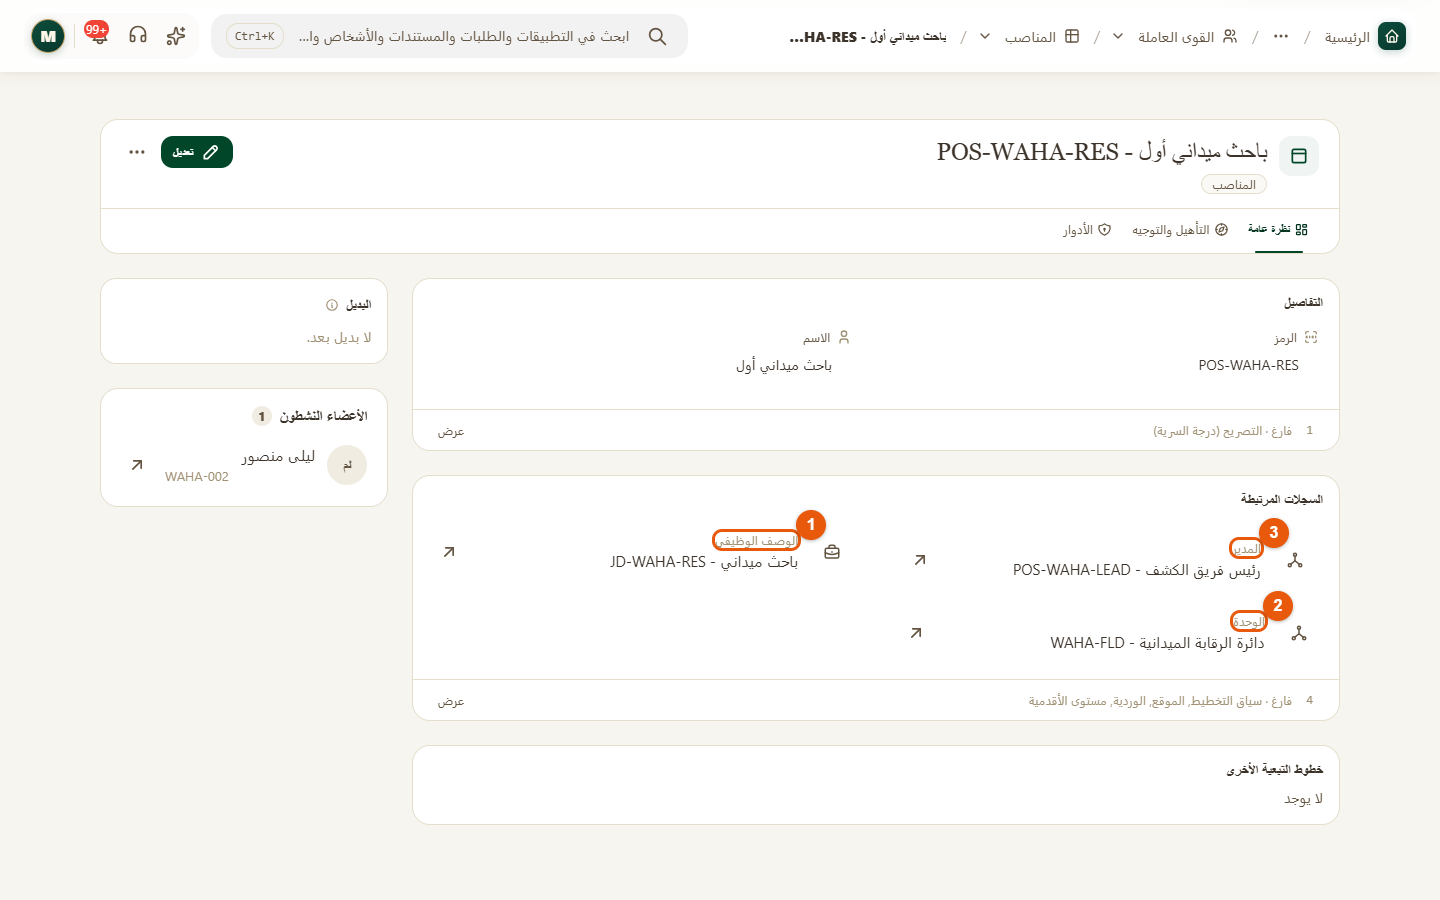
\includegraphics[width=0.95\linewidth]{assets/screens/b-position.png}
\caption{منصب مرتبط بوصفه ووحدته ومديره}
\label{fig:build-position}
\shotnote{تجمع صفحة المنصب ارتباطاته، وتعرض «الأعضاء النشطون» فيه بعد التعيين. ① «الوصف الوظيفي». ② «الوحدة»: الدائرة التي يعمل فيها المنصب. ③ «المدير»: المنصب الأعلى، وبه تُبنى التبعية.}
\end{figure}

\subsection{خطوات العمل والتحقق}
\begin{enumerate}
\item افتح «الموارد البشرية» ← «وصف الوظيفة» ← «سجل جديد»، واكتب «المسمى الوظيفي» و«الرمز الوظيفي»، ثم اضغط «إنشاء». كرّر ذلك لكل وظيفة.
\item افتح «المناصب» ← «سجل جديد»، واكتب «الرمز» و«الاسم».
\item اختر «الوصف الوظيفي» و«الوحدة»، واختر «المدير» إن وُجد، ثم اضغط «إنشاء».
\end{enumerate}

\textbf{تحقق:} افتح منصب الباحث، ويجب أن تظهر الارتباطات الثلاثة تحت «السجلات المرتبطة».

\section{أضف الأعضاء وعيّنهم في مناصبهم}
\label{sec:build-members}

العضو هو حساب الشخص في كيان. أما التعيين فيربطه بمنصب، وبه يعرف النظام عمله. ولا تكتمل خطوة دون الأخرى؛ فالعضو بلا تعيين لا يصل إليه ما يُسند إلى منصبه.

\begin{rcnote}[مثال: مديرية الواحة]
تُضاف ليلى منصور برقم الموظف \en{WAHA-002} و«مقعد كامل». ثم يُنشأ لها تعيين في منصب «باحث ميداني أول»، فتصل إليها كل مهمة تُسند إلى هذا المنصب.
\end{rcnote}

\begin{figure}[H]
\centering
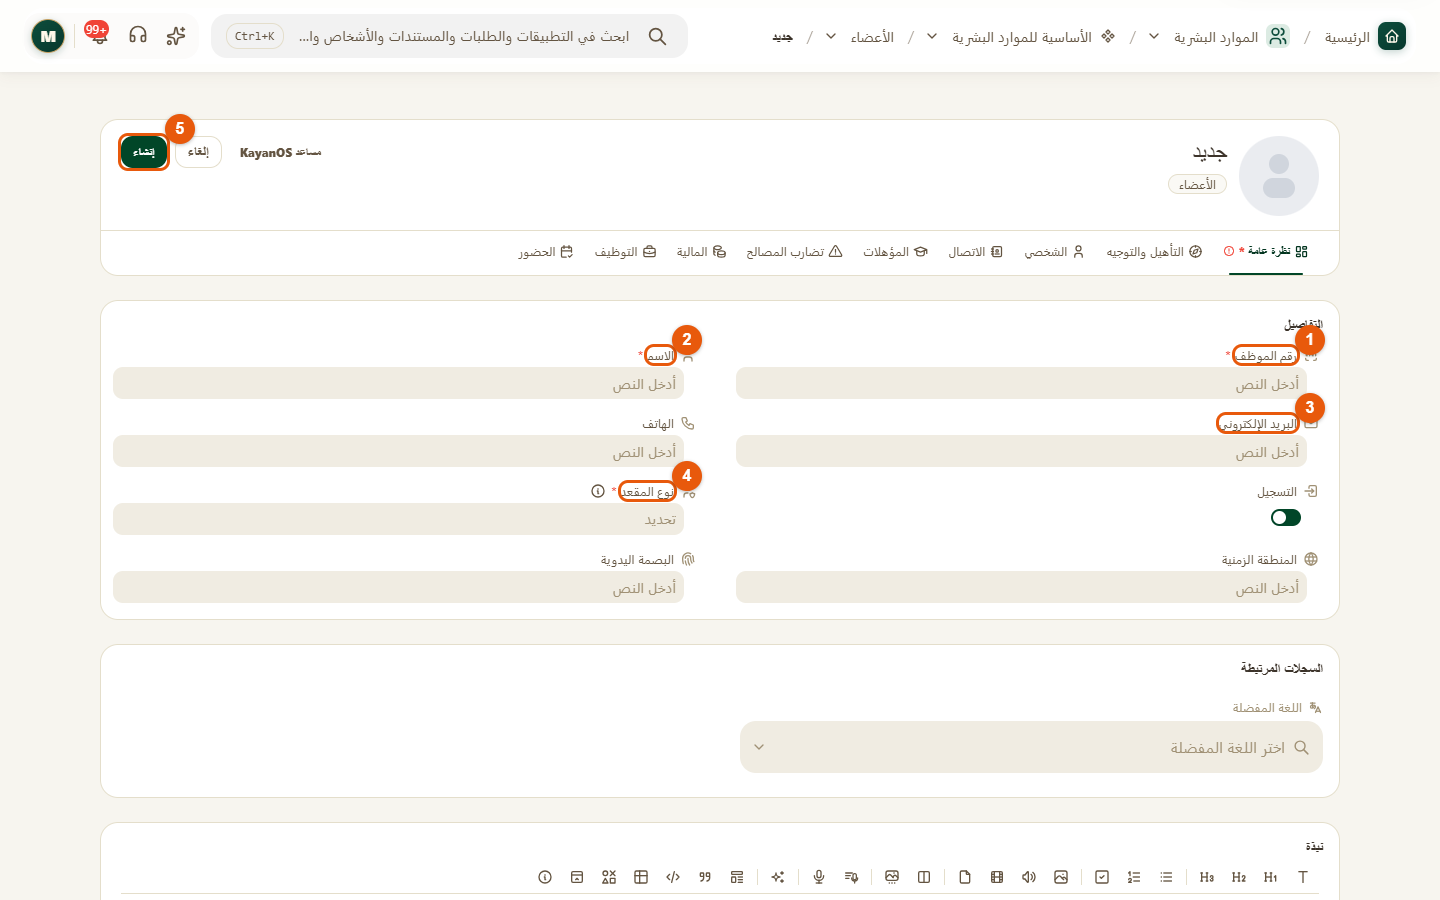
\includegraphics[width=0.95\linewidth]{assets/screens/b-member.png}
\caption{إضافة عضو}
\label{fig:build-member}
\shotnote{الحقول المعلّمة بنجمة مطلوبة، وبقية التبويبات تُستكمل لاحقاً. ① «رقم الموظف». ② «الاسم». ③ «البريد الإلكتروني»: عنوان الدخول. ④ «نوع المقعد»: «مقعد كامل» لمن يعمل في النماذج والموافقات. ⑤ «إنشاء».}
\end{figure}

\begin{figure}[H]
\centering
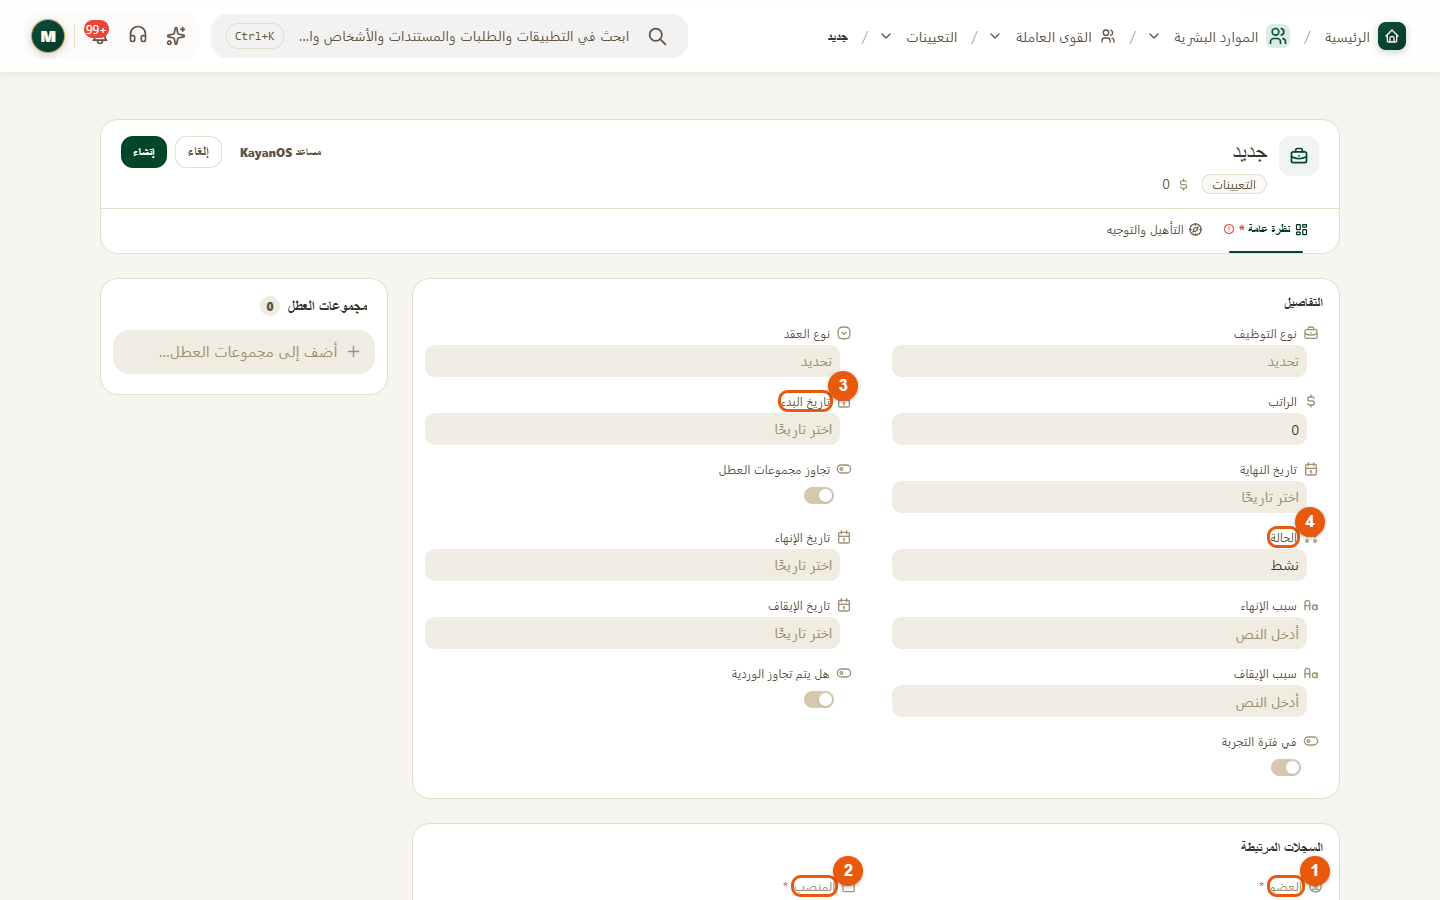
\includegraphics[width=0.95\linewidth]{assets/screens/b-assignment.png}
\caption{إنشاء تعيين}
\label{fig:build-assignment}
\shotnote{التعيين سجل مستقل يحفظ تاريخ العلاقة بين الشخص والمنصب. ① «العضو». ② «المنصب». ③ «تاريخ البدء». ④ «الحالة»: تبدأ «نشط».}
\end{figure}

\subsection{خطوات العمل والتحقق}
\begin{enumerate}
\item افتح «الموارد البشرية» ← «الأعضاء» ← «سجل جديد»، واملأ الحقول المطلوبة، ثم اضغط «إنشاء».
\item افتح «التعيينات» ← «سجل جديد»، واختر «العضو» ثم «المنصب»، ثم اضغط «إنشاء». ويبقى النموذج مفتوحاً بعد الحفظ؛ فافتح «سجل جديد» من القائمة قبل التعيين التالي.
\item لتجرّب بحساب الموظف: افتح العضو، ثم «المزيد من الخيارات» ← «تغيير كلمة المرور». تحتاج كلمة المرور إلى 15 حرفاً على الأقل، ويطلب النظام من الموظف تغييرها عند أول دخول.
\end{enumerate}

\textbf{تحقق:} افتح العضو، ويجب أن يظهر منصبه في «التعيينات النشطة»، ومديره في «التبعية».

\section{أنشئ المجموعات والأدوار}
\label{sec:build-roles}

المجموعة تجمع أشخاصاً لعمل مشترك. أما الدور فيحدد ما يستطيع أصحابه فعله. أسند كل دور إلى \textbf{منصب} لا إلى شخص؛ فإذا تغيّر شاغل المنصب، انتقلت الصلاحية معه دون تعديل.

\begin{rcnote}[مثال: مديرية الواحة]
يُنشأ دور «باحث الواحة» ويُسند إلى منصب «باحث ميداني أول»، ودور «مدقق الواحة» لمنصب «مدقق كشوف»، ودور «رئيس فريق الواحة» لمنصب رئيس الفريق.
\end{rcnote}

\begin{figure}[H]
\centering
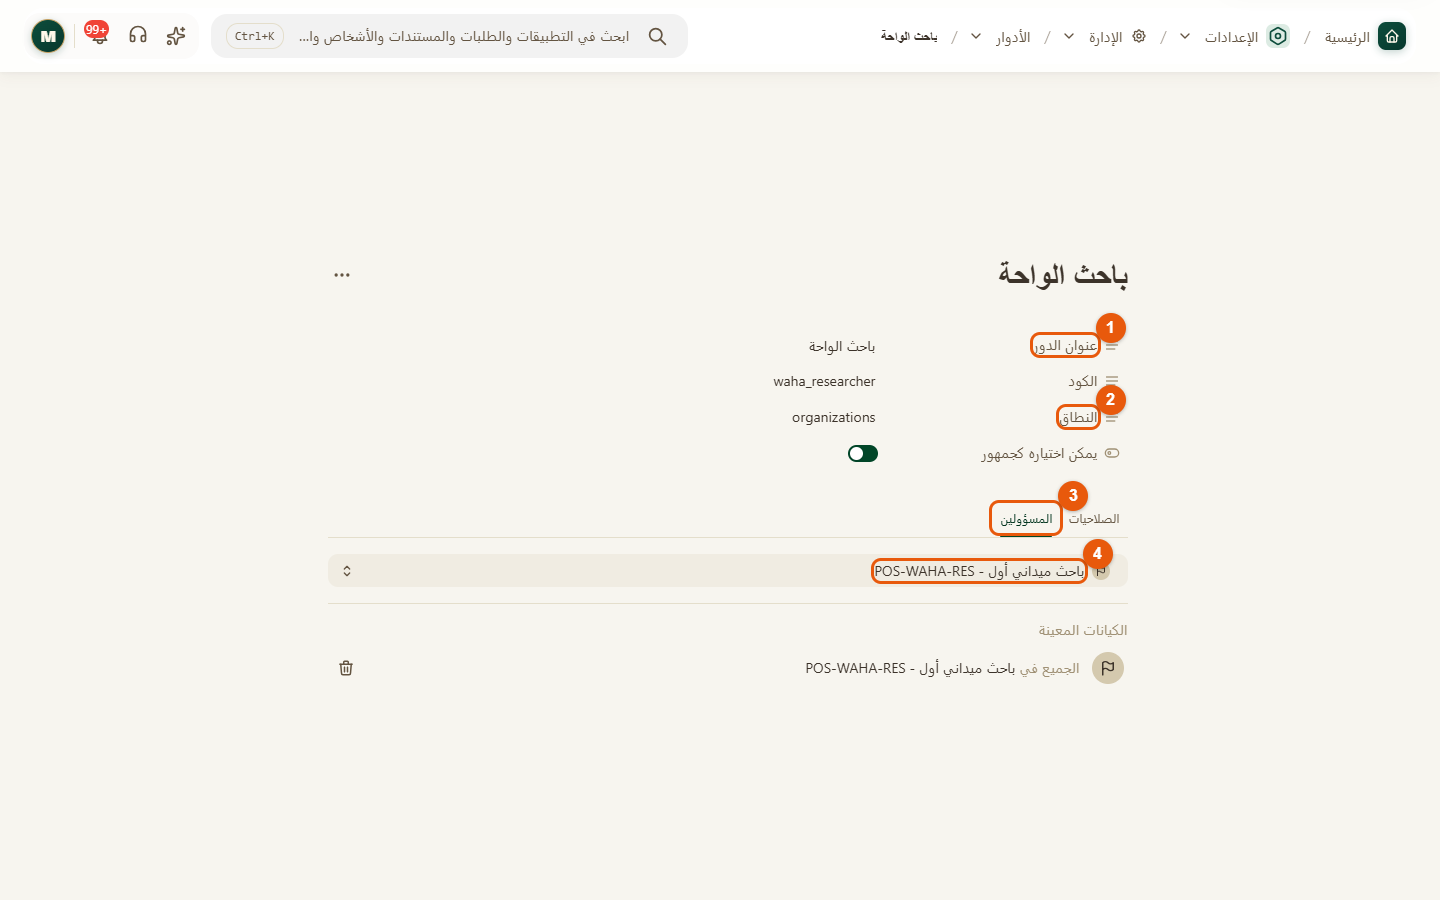
\includegraphics[width=0.95\linewidth]{assets/screens/b-role.png}
\caption{دور مسنَد إلى منصب}
\label{fig:build-role}
\shotnote{يُحفظ الإسناد فور اختياره، ويظهر تحت «الكيانات المعينة». أما الصلاحيات نفسها فتُمنح لاحقاً من نوع السجلات. ① «عنوان الدور». ② «النطاق»: «المنظمات» يعني المؤسسة كلها. ③ «المسؤولين». ④ المنصب الذي يحمل الدور.}
\end{figure}

\subsection{خطوات العمل والتحقق}
\begin{enumerate}
\item للمجموعة: افتح «الموارد البشرية» ← «المجموعات» ← «سجل جديد»، واكتب «الرمز» و«الاسم»، واختر في «نوع المجموعة» «يدوي».
\item للدور: افتح «الإعدادات» ← «الأدوار» ← «إضافة الدور»، واكتب «عنوان الدور» و«الكود»، ثم اضغط «إنشاء الدور».
\item في صفحة الدور افتح «المسؤولين» ← «تعيين الأعضاء والمناصب والعقد»، وابحث عن المنصب واختره.
\end{enumerate}

\textbf{تحقق:} أعد فتح الدور، ويجب أن يبقى المنصب تحت «الكيانات المعينة».

\section{أنشئ التطبيق ونوع السجلات}
\label{sec:build-entity}

التطبيق مكان عمل الفريق، والقسم مجموعة داخله، ونوع السجلات شكل البيانات. وينشأ نوع السجلات مخفياً عن الفريق حتى تحدد تطبيقه وقسمه وتُظهره في التنقل.

\begin{rcnote}[مثال: مديرية الواحة]
تُنشئ المديرية تطبيق «حماية المستهلك - الواحة» وقسم «السجلات»، ثم نوع السجلات «منشآت الواحة» بحقوله العشرة، وأول سجل فيه «فرن السنابل» في «المزة».
\end{rcnote}

\begin{table}[H]
\centering
\caption{حقول «منشآت الواحة»}
\label{tab:build-fields}
\begin{tabularx}{\linewidth}{R{3.6cm} R{2.4cm} Y}
\rcHeaderRow
\thh{العنوان} & \thh{النوع} & \thh{ملاحظة}\\
اسم المنشأة & نص & مطلوب، ويُختار «حقلاً للاسم المعروض».\\
رقم السجل التجاري & نص & \\
النشاط & اختيار & فرن، مطعم، مواد غذائية، أخرى.\\
المحافظة & اختيار & المحافظات السورية الأربع عشرة.\\
العنوان التفصيلي & نص & يحدّثه الكشف بعد الاعتماد.\\
الموقع على الخريطة & موقع & \\
حالة التوثيق & اختيار & غير موثقة، موثقة.\\
تاريخ التوثيق & تاريخ ووقت & \\
المعتمد بواسطة & اختيار عضو & لا يكتبه النموذج؛ يُملأ يدوياً أو بإجراء آلي.\\
مرجع الكشف المعتمد & نص & \\
\end{tabularx}
\end{table}

\begin{figure}[H]
\centering
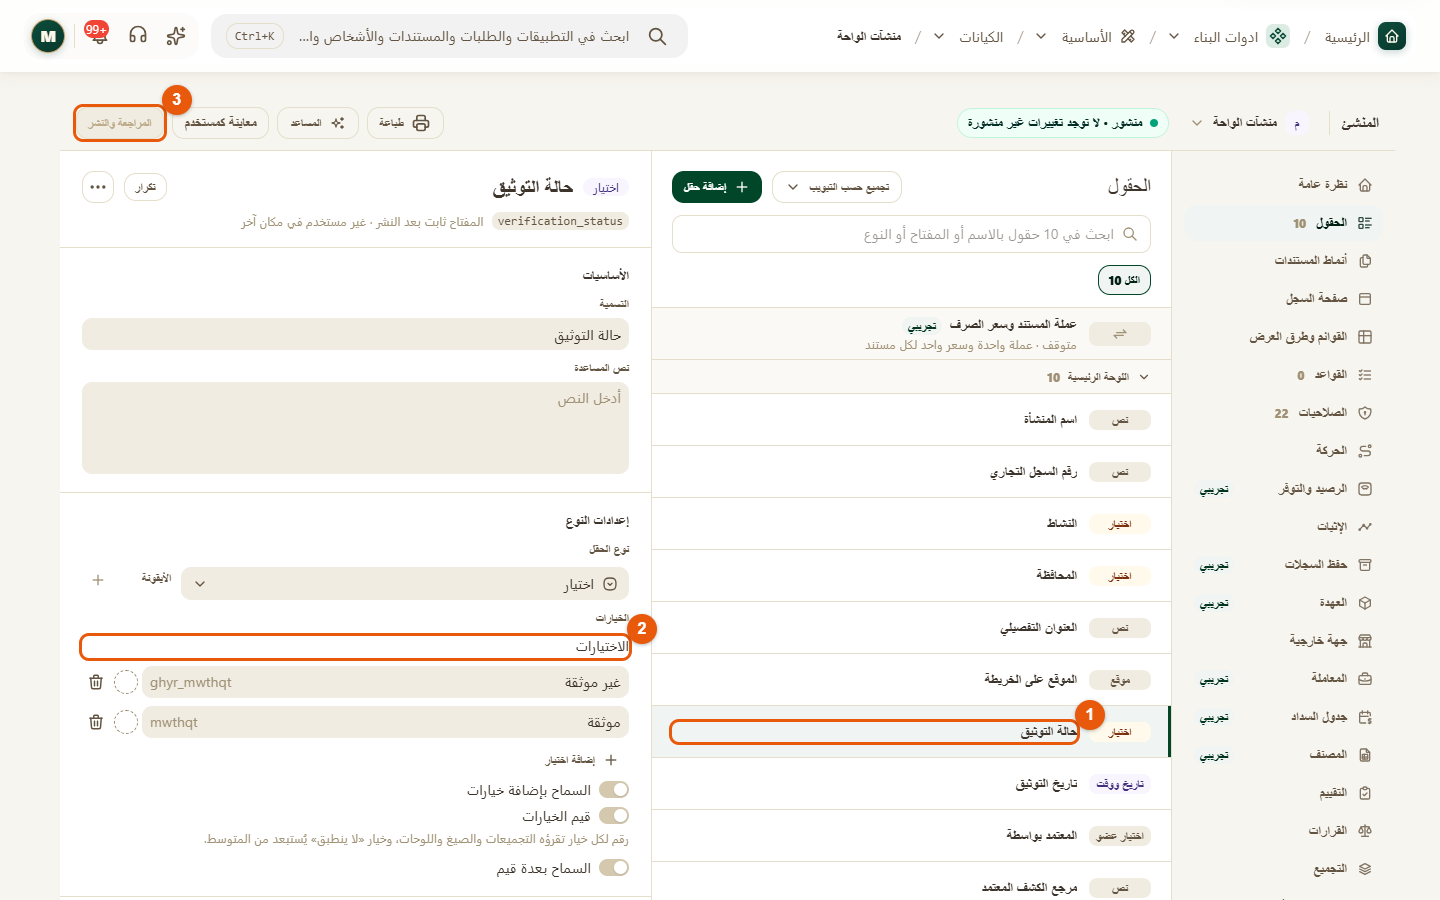
\includegraphics[width=0.95\linewidth]{assets/screens/b-entity-fields.png}
\caption{حقل اختيار ومفاتيح خياراته}
\label{fig:build-entity-fields}
\shotnote{يحفظ النظام كل خيار بمفتاح يولّده من نصه بحروف لاتينية، فيُحفظ «موثقة» بالمفتاح mwthqt و«دمشق» بالمفتاح dmshq. وستحتاج إلى هذا المفتاح، لا إلى النص، في القيم الافتراضية والقواعد. ① الحقل المحدد. ② «الاختيارات»: يظهر المفتاح بجانب كل خيار. ③ «المراجعة والنشر».}
\end{figure}

\subsection{خطوات العمل والتحقق}
\begin{enumerate}
\item افتح «ادوات البناء» ← «التطبيقات» ← «سجل جديد»، واملأ «العنوان» و«الوصف» و«الأيقونة»، ثم اضغط «إنشاء». والأيقونة اسم إنجليزي قصير مثل \en{shield}.
\item افتح «أقسام التطبيق» ← «سجل جديد»، واكتب «العنوان» و«الوصف» و«الأيقونة»، واختر «التطبيق»، ثم اضغط «إنشاء».
\item افتح «الكيانات» ← «إضافة كيان»، واكتب «عنوان الكيان» والوصف.
\item اضغط «حقل 1» لتفتح «إعدادات الحقل» على الجانب، واختر النوع، واكتب العنوان والمفتاح بحروف إنجليزية. ثم اضغط «اضافة حقل جديد» لكل حقل آخر، و«إضافة اختيار» لكل خيار.
\item اضغط «إعدادات الكيان»، واختر في «حقول الاسم المعروض» «اسم المنشأة»، وفعّل «إظهار في التنقل»، واختر «التطبيق» و«قسم التطبيق»، ثم اضغط «انشاء كيان».
\item افتح التطبيق، واضغط «سجل جديد» تحت «منشآت الواحة»، وأدخل أول منشأة.
\end{enumerate}

\textbf{تحقق:} يجب أن يظهر «منشآت الواحة» في صفحة التطبيق، وأن يفتح سجل المنشأة بقيمه. وإذا لم يظهر، فراجع «إظهار في التنقل» والقسم.

\section{امنح الأدوار صلاحية نوع السجلات}
\label{sec:build-grants}

لا يرى أحد سجلات المنشآت حتى يحمل دوراً يمنحه «قائمة» و«فتح». وتُحفظ الصلاحيات هنا كمسودة، فلا تعمل حتى تنشرها.

\begin{rcnote}[مثال: مديرية الواحة]
تمنح المديرية الأدوار الثلاثة «قائمة» و«فتح» فقط. أما تحديث المنشأة فيجري بالنموذج بعد الاعتماد، لا بيد الباحث.
\end{rcnote}

\begin{figure}[H]
\centering
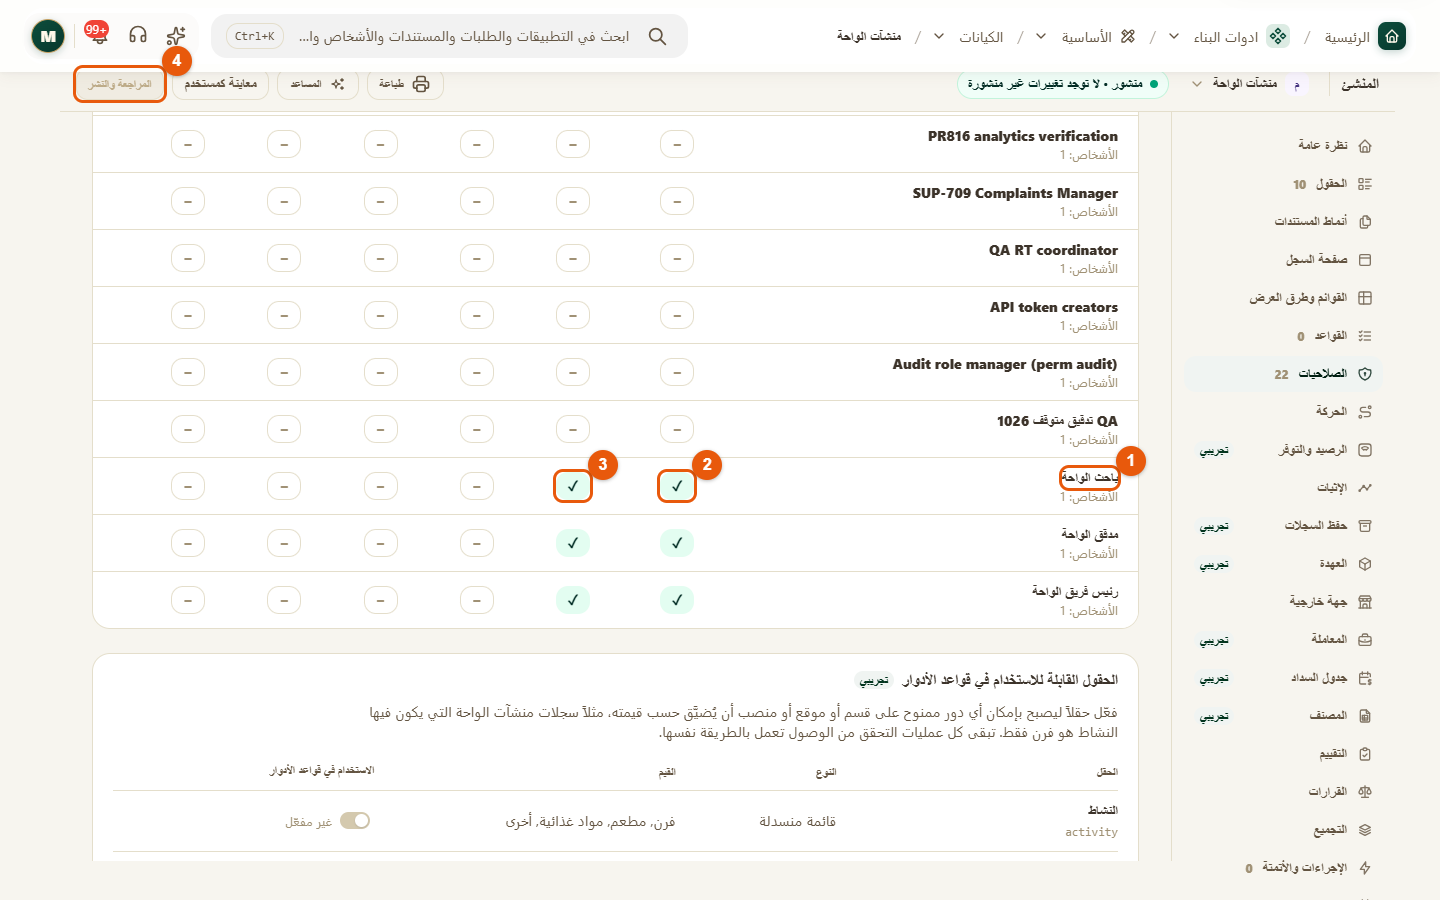
\includegraphics[width=0.95\linewidth]{assets/screens/b-grants.png}
\caption{صلاحيات الأدوار على نوع السجلات}
\label{fig:build-grants}
\shotnote{كل صف دور، وكل عمود فعل. ويُظهر الصف عدد الأشخاص الذين يحملون الدور، وهو دليل على صحة الإسناد إلى المنصب. ① الدور. ② «قائمة». ③ «فتح». ④ «المراجعة والنشر»: يعرض التغييرات قبل نشرها.}
\end{figure}

\subsection{خطوات العمل والتحقق}
\begin{enumerate}
\item افتح «الكيانات» ← نوع السجلات ← «الصلاحيات» ← «الأدوار».
\item اضغط «قائمة» و«فتح» في صف كل دور.
\item اضغط «المراجعة والنشر»، ثم «نشر».
\end{enumerate}

\textbf{تحقق:} يجب أن تتحول الحالة أعلى الصفحة إلى «منشور · لا توجد تغييرات غير منشورة».

\section{أنشئ النموذج واربطه بالمنشأة}
\label{sec:build-form}

يبدأ النموذج بسؤال يختار المنشأة، ثم بأسئلة تقرأ بياناتها وتكتب إليها. ويضيف المعالج هذه الأسئلة دفعة واحدة، ويحدد لكل حقل هل يُقرأ أم يُكتب أم الاثنين معاً.

\begin{rcnote}[مثال: مديرية الواحة]
في «كشف منشأة - الواحة» يُقرأ الاسم والرقم والنشاط ولا تُعدّل. ويُقرأ العنوان والمحافظة ويُكتبان بعد الاعتماد. أما «حالة التوثيق» فمخفية، وتُكتب «موثقة» بعد الاعتماد.
\end{rcnote}

\begin{figure}[H]
\centering
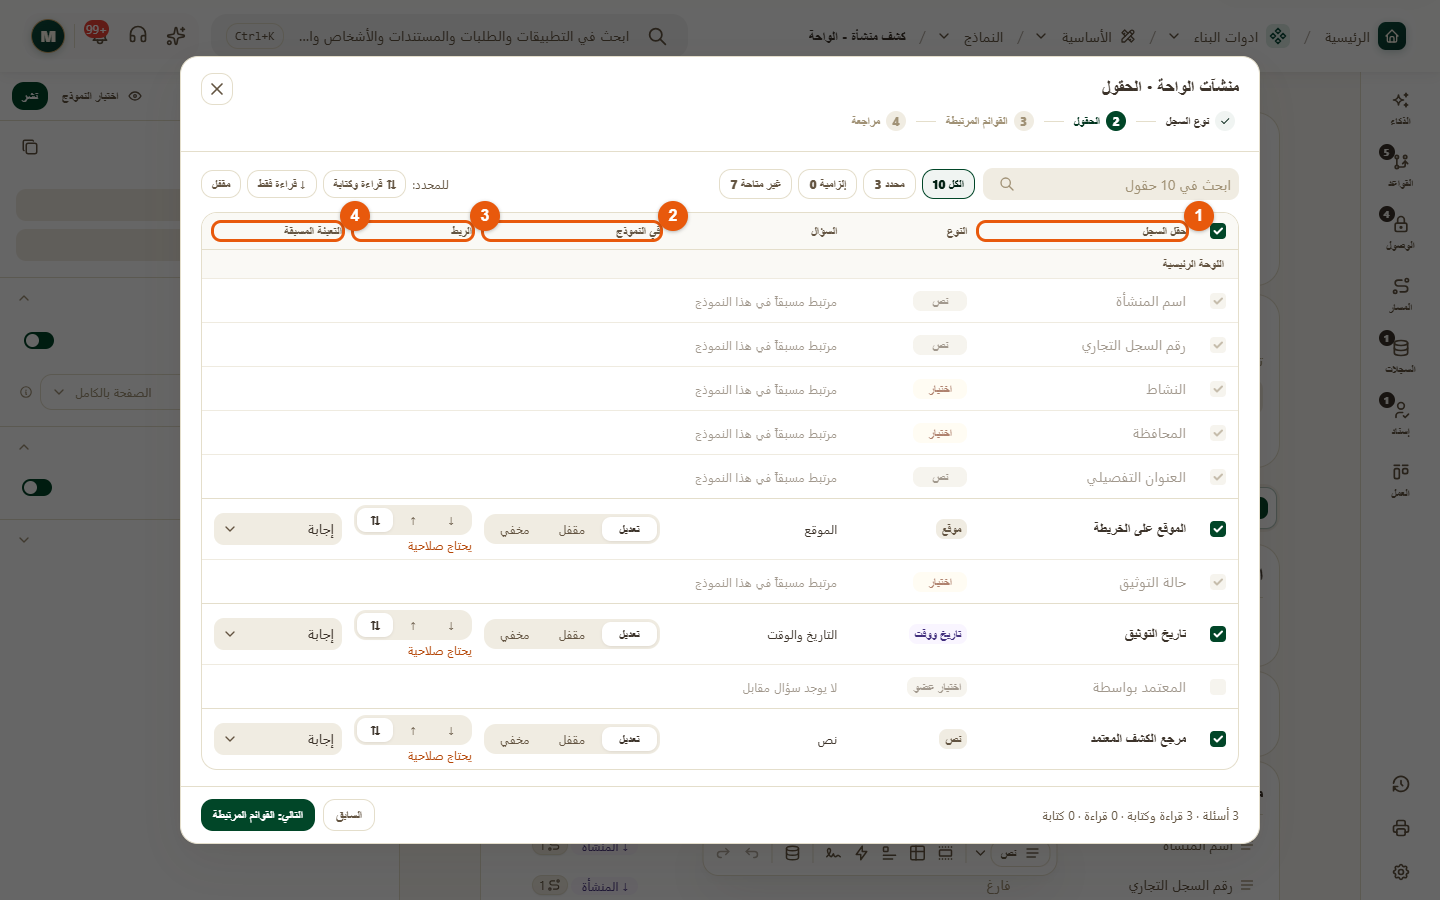
\includegraphics[width=0.95\linewidth]{assets/screens/b-wizard.png}
\caption{معالج «إضافة أسئلة من نوع سجل»}
\label{fig:build-wizard}
\shotnote{يعرض كل صف حقلاً من المنشأة، ويحدد ما يحدث له في النموذج. ① «حقل السجل». ② «في النموذج»: «تعديل» أو «مقفل» أو «مخفي». ③ «الربط»: ↓ قراءة، ↑ كتابة، ⇅ الاثنان. ④ «التعبئة المسبقة».}
\end{figure}

\begin{figure}[H]
\centering
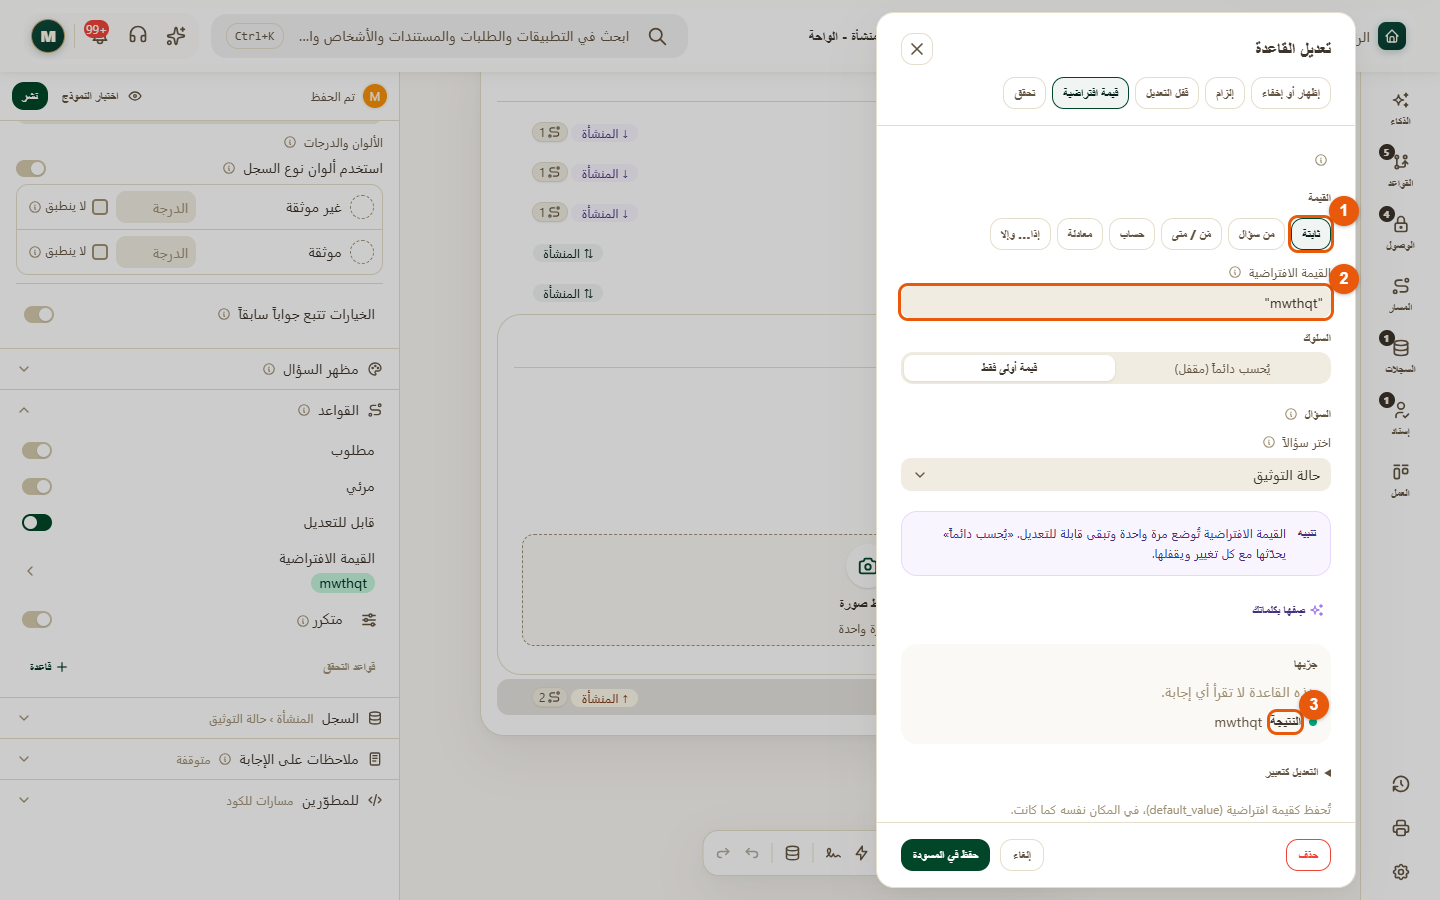
\includegraphics[width=0.85\linewidth]{assets/screens/b-default.png}
\caption{قيمة افتراضية لسؤال مخفي}
\label{fig:build-default}
\shotnote{القيمة هنا تعبير، لذلك يُكتب النص بين علامتي تنصيص. ويجب أن يكون مفتاح الخيار، لا نصه الظاهر. ① «ثابتة». ② «القيمة الافتراضية»: \en{"mwthqt"}. ③ «النتيجة»: تتحقق منها قبل الحفظ.}
\end{figure}

\subsection{خطوات العمل والتحقق}
\begin{enumerate}
\item افتح «ادوات البناء» ← «النماذج» ← «إنشاء نموذج». اكتب الاسم و«كود النموذج» و«الاختصار المرجعي»، مثل \en{KSHF}، فتحمل الكشوف أرقاماً مثل \en{KSHF-1}. ثم اختر التطبيق والقسم، واضغط «إنشاء».
\item افتح «السجلات» في الشريط الجانبي، واضغط «سؤال سجل»، واختر في «نوع السجل» «منشآت الواحة». وسمِّ السؤال «المنشأة».
\item افتح «السجلات» مرة أخرى، واضغط «من نوع سجل». اختر نوع السجلات، ثم استخدم سؤال «المنشأة» الموجود، وحدّد الحقول وطريقة ربطها، ثم اضغط «إضافة».
\item أضف أسئلة الكشف من الشريط السفلي: «اختر نوع الحقل» يضيف سؤالاً جديداً من النوع الذي تختاره، ولا يغيّر نوع السؤال المحدد.
\item حدّد سؤال «حالة التوثيق»، ثم «القواعد» ← «القيمة الافتراضية» ← «ثابتة»، واكتب \en{"mwthqt"}. وتأكد من أن «متكرر» متوقف.
\end{enumerate}

\textbf{تحقق:} افتح «السجلات» في الشريط الجانبي، ويجب أن تظهر بطاقة «المنشأة» وتحتها الحقول المرتبطة بأسهمها.

\section{اسمح للنموذج بالكتابة إلى المنشأة}
\label{sec:build-allow}

الكتابة إلى سجل يملكه غيرك تحتاج إلى موافقة صاحبه. وما دامت الموافقة معلّقة، يُعتمد الكشف ولا تتغير المنشأة. لذلك لا تتخطَّ هذه الخطوة.

\begin{rcnote}[مثال: مديرية الواحة]
بعد إضافة الأسئلة ظهر في لوحة «السجلات» «بانتظار موافقة مسؤول «منشآت الواحة»». فوافق مسؤول النظام على الحقول الثلاثة التي يكتبها الكشف.
\end{rcnote}

\begin{figure}[H]
\centering
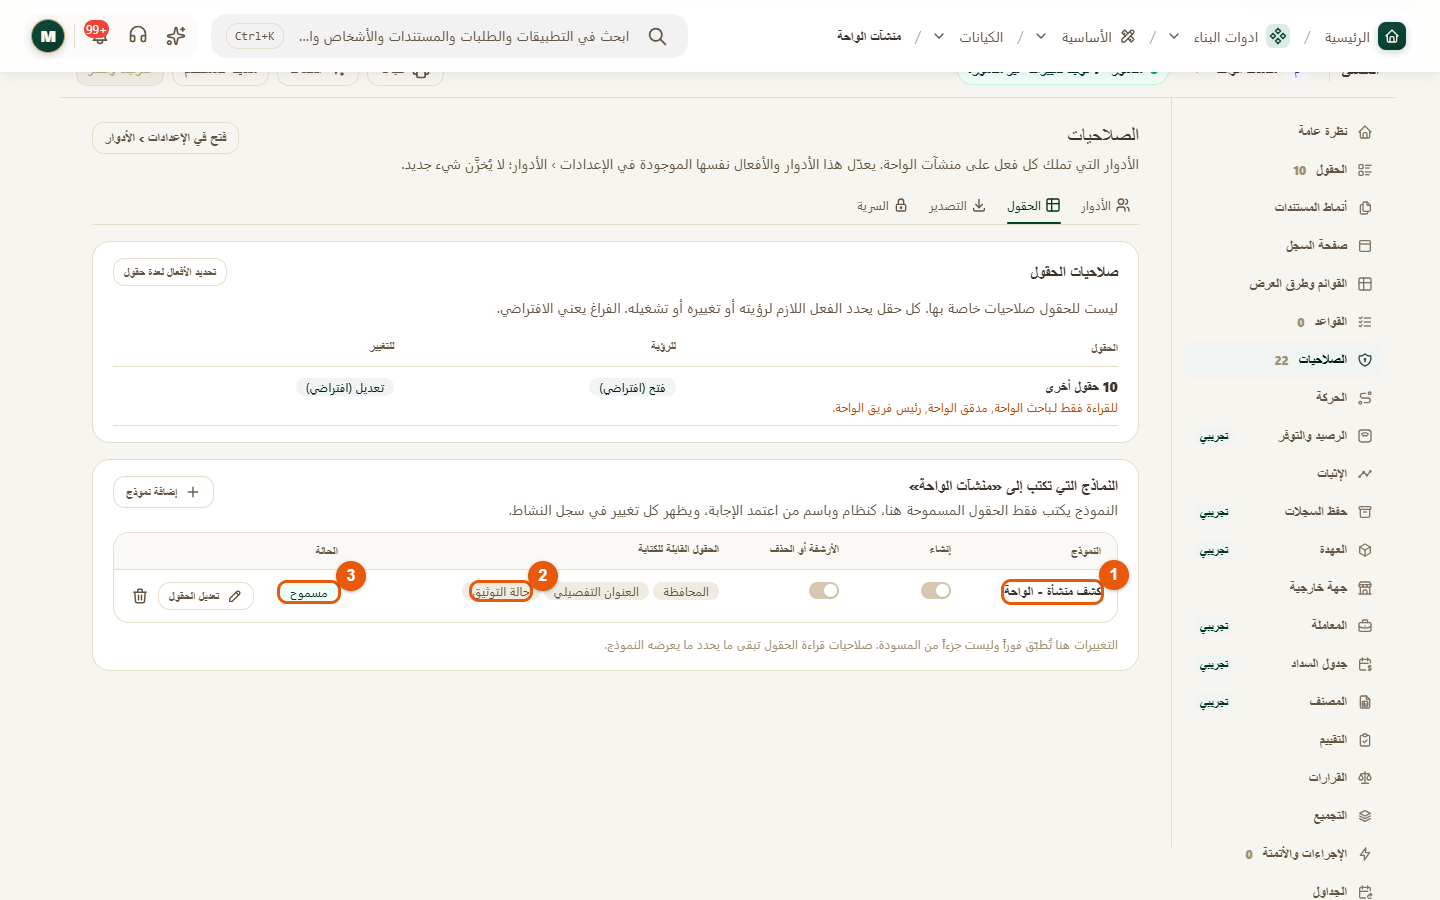
\includegraphics[width=0.95\linewidth]{assets/screens/b-form-writes.png}
\caption{«النماذج التي تكتب إلى «منشآت الواحة»»}
\label{fig:build-allow}
\shotnote{يكتب النموذج الحقول المسموح بها هنا فقط، ويُسجَّل كل تغيير باسم من اعتمد الإجابة. ① النموذج. ② «الحقول القابلة للكتابة». ③ «الحالة»: «مسموح» بعد الموافقة.}
\end{figure}

\subsection{خطوات العمل والتحقق}
\begin{enumerate}
\item في لوحة «السجلات» داخل النموذج، اضغط «السماح في نوع السجل».
\item راجع الحقول، ثم اضغط «موافقة».
\end{enumerate}

\textbf{تحقق:} يجب أن تتحول حالة الطلب إلى «مسموح».

\section{ابنِ المسار وخطوة الموافقة}
\label{sec:build-journey}

يضيف «تفعيل المسار» سبع حالات جاهزة، منها «مُرسل» و«مقبول» و«مرفوض» و«بحاجة لاستكمال». وما عليك إلا أن تضيف خطوة الموافقة وتحدد أين تنقل كل نتيجة.

\begin{rcnote}[مثال: مديرية الواحة]
تعمل «تدقيق الكشف» في حالة «مُرسل» وتبدأ وحدها، ويوقّع فيها منصب «مدقق كشوف». وتنقل نتائجها الكشف إلى «مقبول» أو «مرفوض» أو «بحاجة لاستكمال».
\end{rcnote}

\begin{figure}[H]
\centering
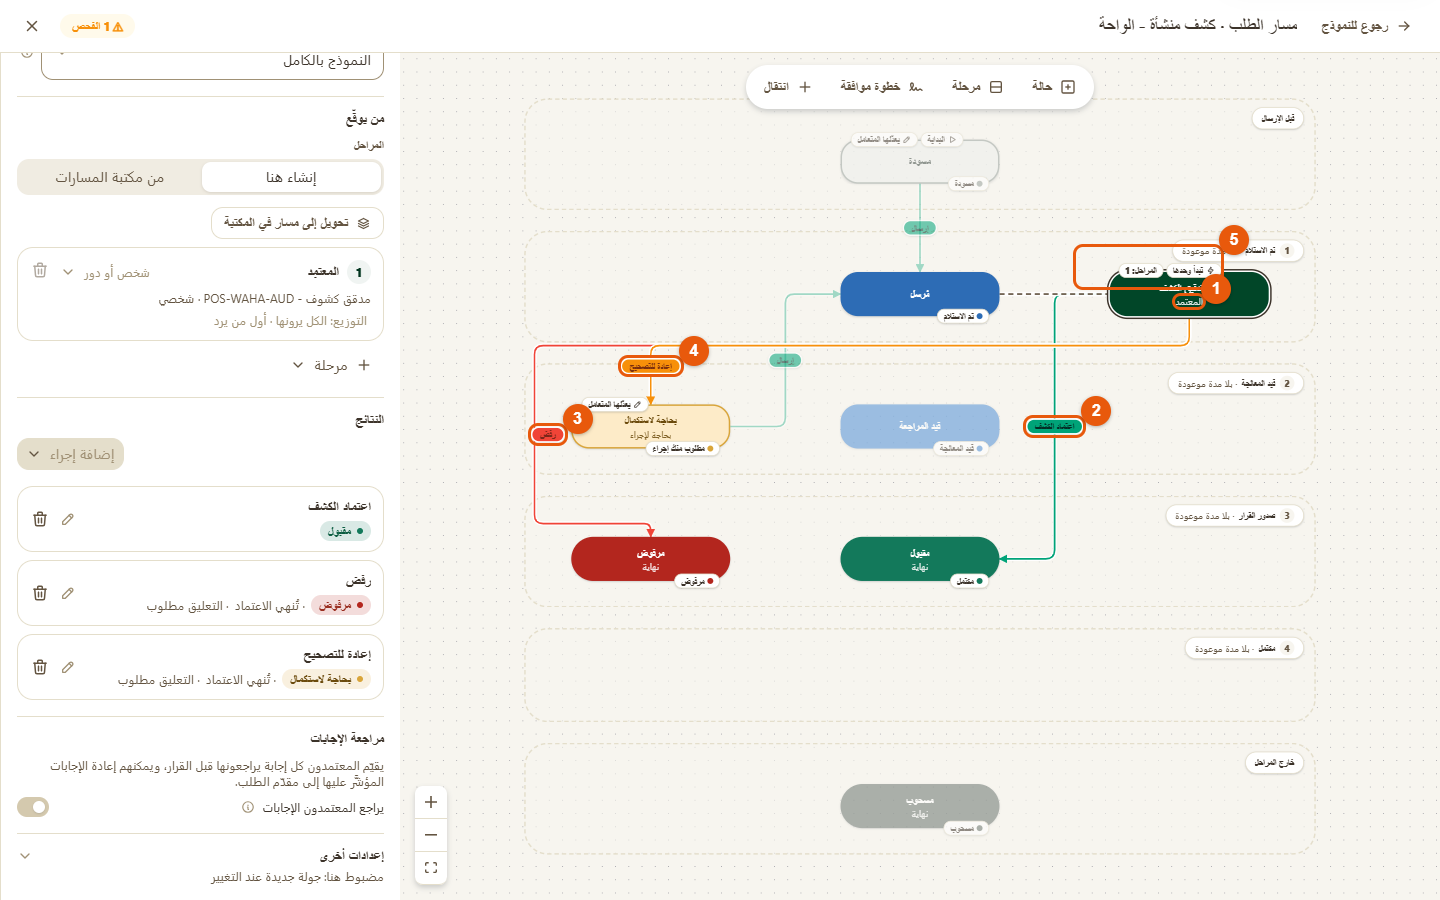
\includegraphics[width=0.95\linewidth]{assets/screens/b-journey.png}
\caption{خطوة الموافقة ونتائجها الثلاث}
\label{fig:build-journey}
\shotnote{تظهر كل نتيجة على الخريطة سهماً بلونها. وإذا بقيت النتيجة «تبقى الحالة»، فلن يتغير الكشف بعد القرار. ① المنصب الذي يوقّع. ② «اعتماد الكشف» إلى «مقبول». ③ «رفض» إلى «مرفوض»، والتعليق مطلوب. ④ «إعادة للتصحيح» إلى «بحاجة لاستكمال». ⑤ الخطوة على الخريطة.}
\end{figure}

\subsection{خطوات العمل والتحقق}
\begin{enumerate}
\item افتح «المسار» ← «تفعيل المسار»، ثم «تفعيل خطوات الموافقة»، ثم «خطوة موافقة».
\item اكتب الاسم. ثم اضغط «تغيير» تحت «تعمل في»، واختر «مُرسل» وحدها، واختر في «تبدأ» «عند الوصول إلى حالتها».
\item في «من يوقّع» افتح «المعتمِد» ← «محدد العضوية»، واختر المنصب.
\item في «النتائج» افتح «موافقة»، وسمّها «اعتماد الكشف»، واجعل «تنقل الطلب إلى» «مقبول». وافتح «رفض»، واجعلها «مرفوض» والتعليق «مطلوب».
\item اضغط «إضافة إجراء» ← «طلب تغييرات»، وسمّه «إعادة للتصحيح»، واجعل «تنقل الطلب إلى» «بحاجة لاستكمال».
\item اختر في «التوقيع» «مطلوب» إذا كان لدى المدققين مفاتيح توقيع، وإلا فاختر «غير مطلوب».
\end{enumerate}

\textbf{تحقق:} يجب أن تظهر ثلاثة أسهم من الخطوة، وألا يذكر «الفحص» خطوة بلا موقّع.

\section{حدّد الوصول وفعّل التكليف ثم انشر}
\label{sec:build-access}

يحدد «الوصول» من يرى الكشوف ويرسلها. ويسمح «إسناد» بتكليف الباحثين بالنموذج. ولا يصل أي من ذلك إلى الفريق قبل النشر.

\begin{rcnote}[مثال: مديرية الواحة]
يحصل الباحثون على «قائمة» و«فتح» و«إرسال الطلبات»، ويحصل المدققون ورئيس الفريق على «قائمة» و«فتح». ثم يُفعَّل التكليف ويُنشر النموذج.
\end{rcnote}

\begin{figure}[H]
\centering
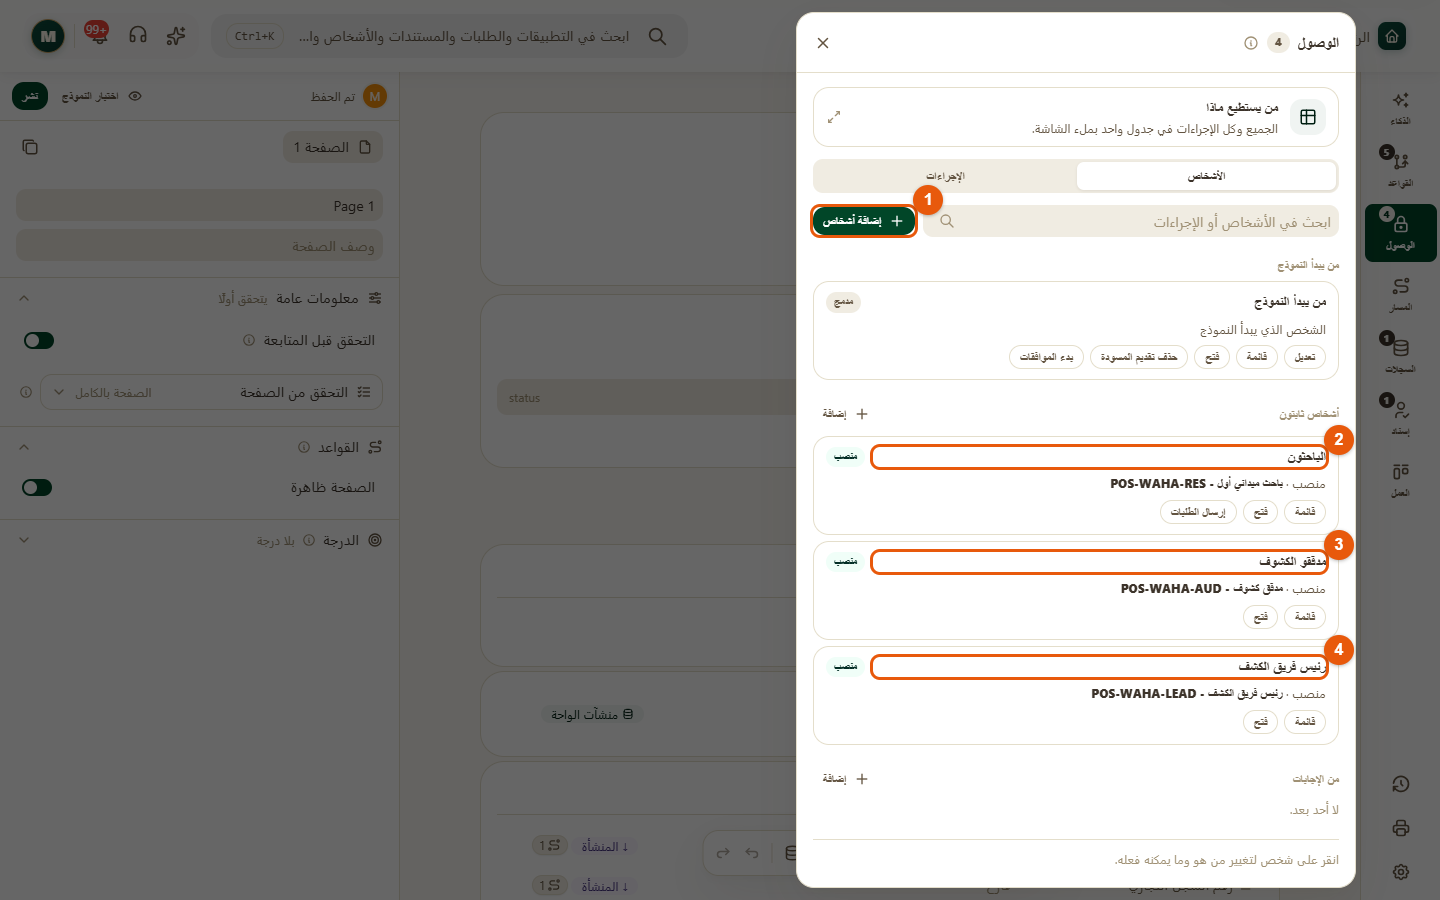
\includegraphics[width=0.85\linewidth]{assets/screens/b-access.png}
\caption{الوصول إلى النموذج}
\label{fig:build-access}
\shotnote{كل بطاقة دور للنموذج، مسنَد إلى منصب، وتحته إجراءاته. ① «إضافة أشخاص». ② الباحثون. ③ المدققون. ④ رئيس الفريق.}
\end{figure}

\subsection{خطوات العمل والتحقق}
\begin{enumerate}
\item افتح «الوصول» ← «إضافة» بجانب «أشخاص ثابتون». اكتب الاسم، واختر المنصب في «من»، وحدّد الإجراءات، ثم اضغط «حفظ في المسودة».
\item افتح «إسناد»، وفعّل «يمكن التكليف به».
\item اضغط «نشر»، وراجع التغييرات، ثم اضغط «نشر».
\end{enumerate}

\textbf{تحقق:} يجب أن يظهر النموذج في «قائمة النماذج» بإصدار منشور.

\section{أطلق خطة التكليف}
\label{sec:build-plan}

الخطة هي التي توصل الكشف إلى الباحثين. وتعرض قبل الإطلاق معاينة تبيّن لمن سيصل كل سجل، فتكشف أي خطأ في المناصب أو التعيينات.

\begin{rcnote}[مثال: مديرية الواحة]
تعرض المعاينة: «فرن السنابل» ← «باحث ميداني أول» ← «ليلى منصور». وهذا يثبت أن المنصب والتعيين والدور مضبوطة كلها.
\end{rcnote}

\begin{figure}[H]
\centering
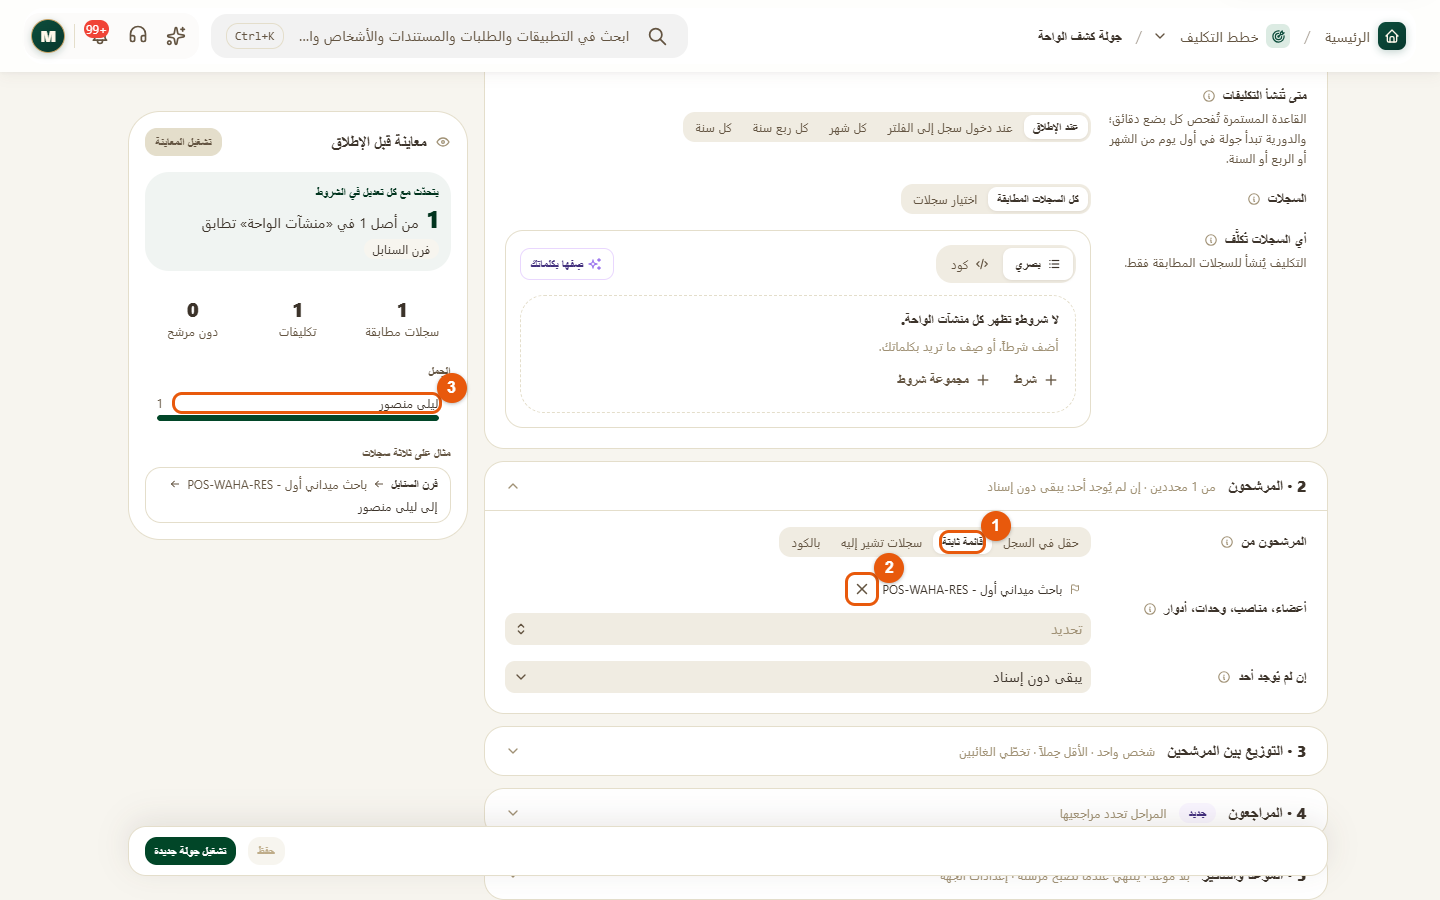
\includegraphics[width=0.95\linewidth]{assets/screens/b-plan.png}
\caption{المرشحون ومعاينة الخطة}
\label{fig:build-plan}
\shotnote{تحسب المعاينة كل تكليف قبل إنشائه. وإذا ظهر سجل «دون مرشح»، فراجع التعيين أو المنصب. ① «قائمة ثابتة». ② المنصب المرشَّح. ③ الشخص الذي سيصله التكليف.}
\end{figure}

\subsection{خطوات العمل والتحقق}
\begin{enumerate}
\item افتح «خطط التكليف» ← «خطة جديدة»، واختر النموذج، واكتب «اسم الخطة»، ثم اضغط «إنشاء والإعداد». وإذا ظهر «التكليف متوقف لهذا النموذج»، فاضغط «تشغيل التكليف».
\item افتح «2 · المرشحون»، واختر «قائمة ثابتة»، ثم أضف المنصب.
\item اضغط «تشغيل المعاينة»، ثم «حفظ»، ثم «إنشاء التكليفات».
\end{enumerate}

\textbf{تحقق:} يجب أن تصبح الخطة «نشطة»، وأن يظهر في «نظرة عامة» عدد «مُسندة».

\section{شغّل الكشف بحساب الباحث}
\label{sec:build-run-researcher}

يدخل الباحث بحسابه، فيجد التكليف في الصفحة الرئيسية. ويفتح الكشف والمنشأة محددة فيه، ثم يرسله إلى التدقيق.

\begin{rcnote}[مثال: مديرية الواحة]
تجد ليلى «1 تكليفات مطلوبة منك». تفتح «فرن السنابل»، وتكمل العنوان إلى «المزة، شارع الجلاء، بناء 12»، وتوصي بالتوثيق، ثم ترسل الكشف.
\end{rcnote}

\begin{figure}[H]
\centering
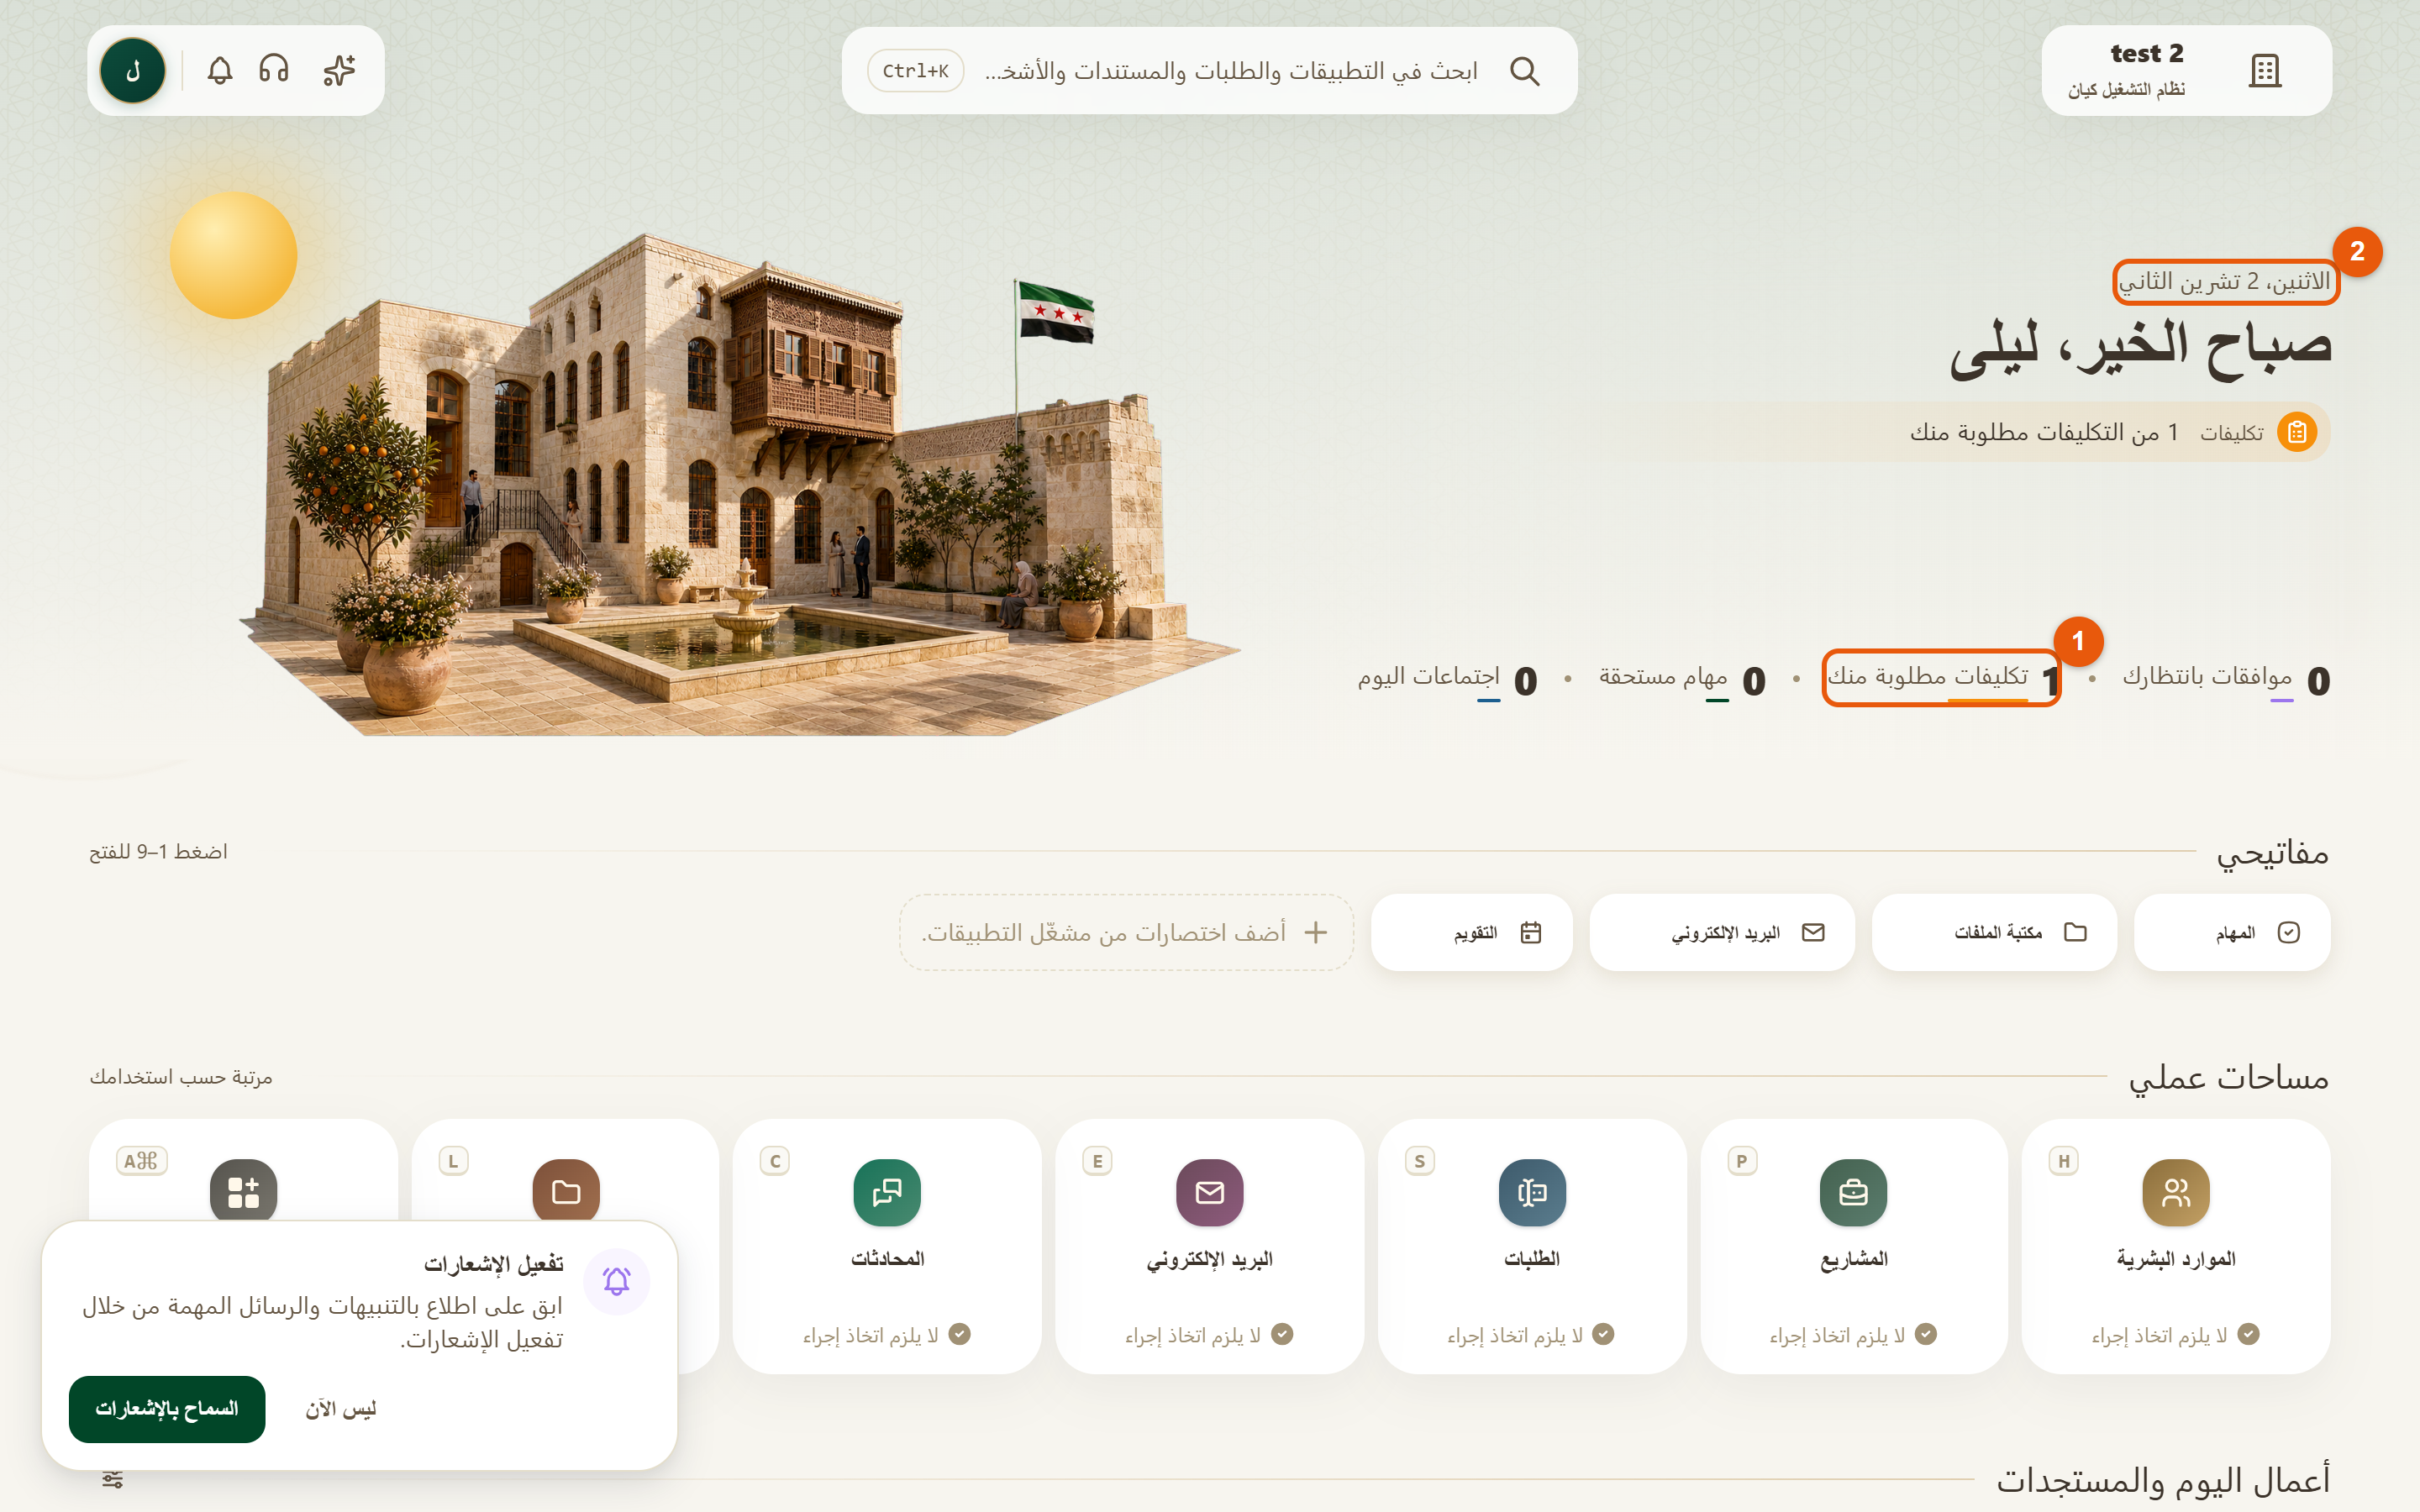
\includegraphics[width=0.95\linewidth]{assets/screens/b-laila-home.png}
\caption{الصفحة الرئيسية للباحث}
\label{fig:build-laila-home}
\shotnote{تجمع الصفحة الرئيسية ما ينتظر الموظف، ويظهر التاريخ بالأشهر الشامية. ① «تكليفات مطلوبة منك». ② التاريخ.}
\end{figure}

\begin{figure}[H]
\centering
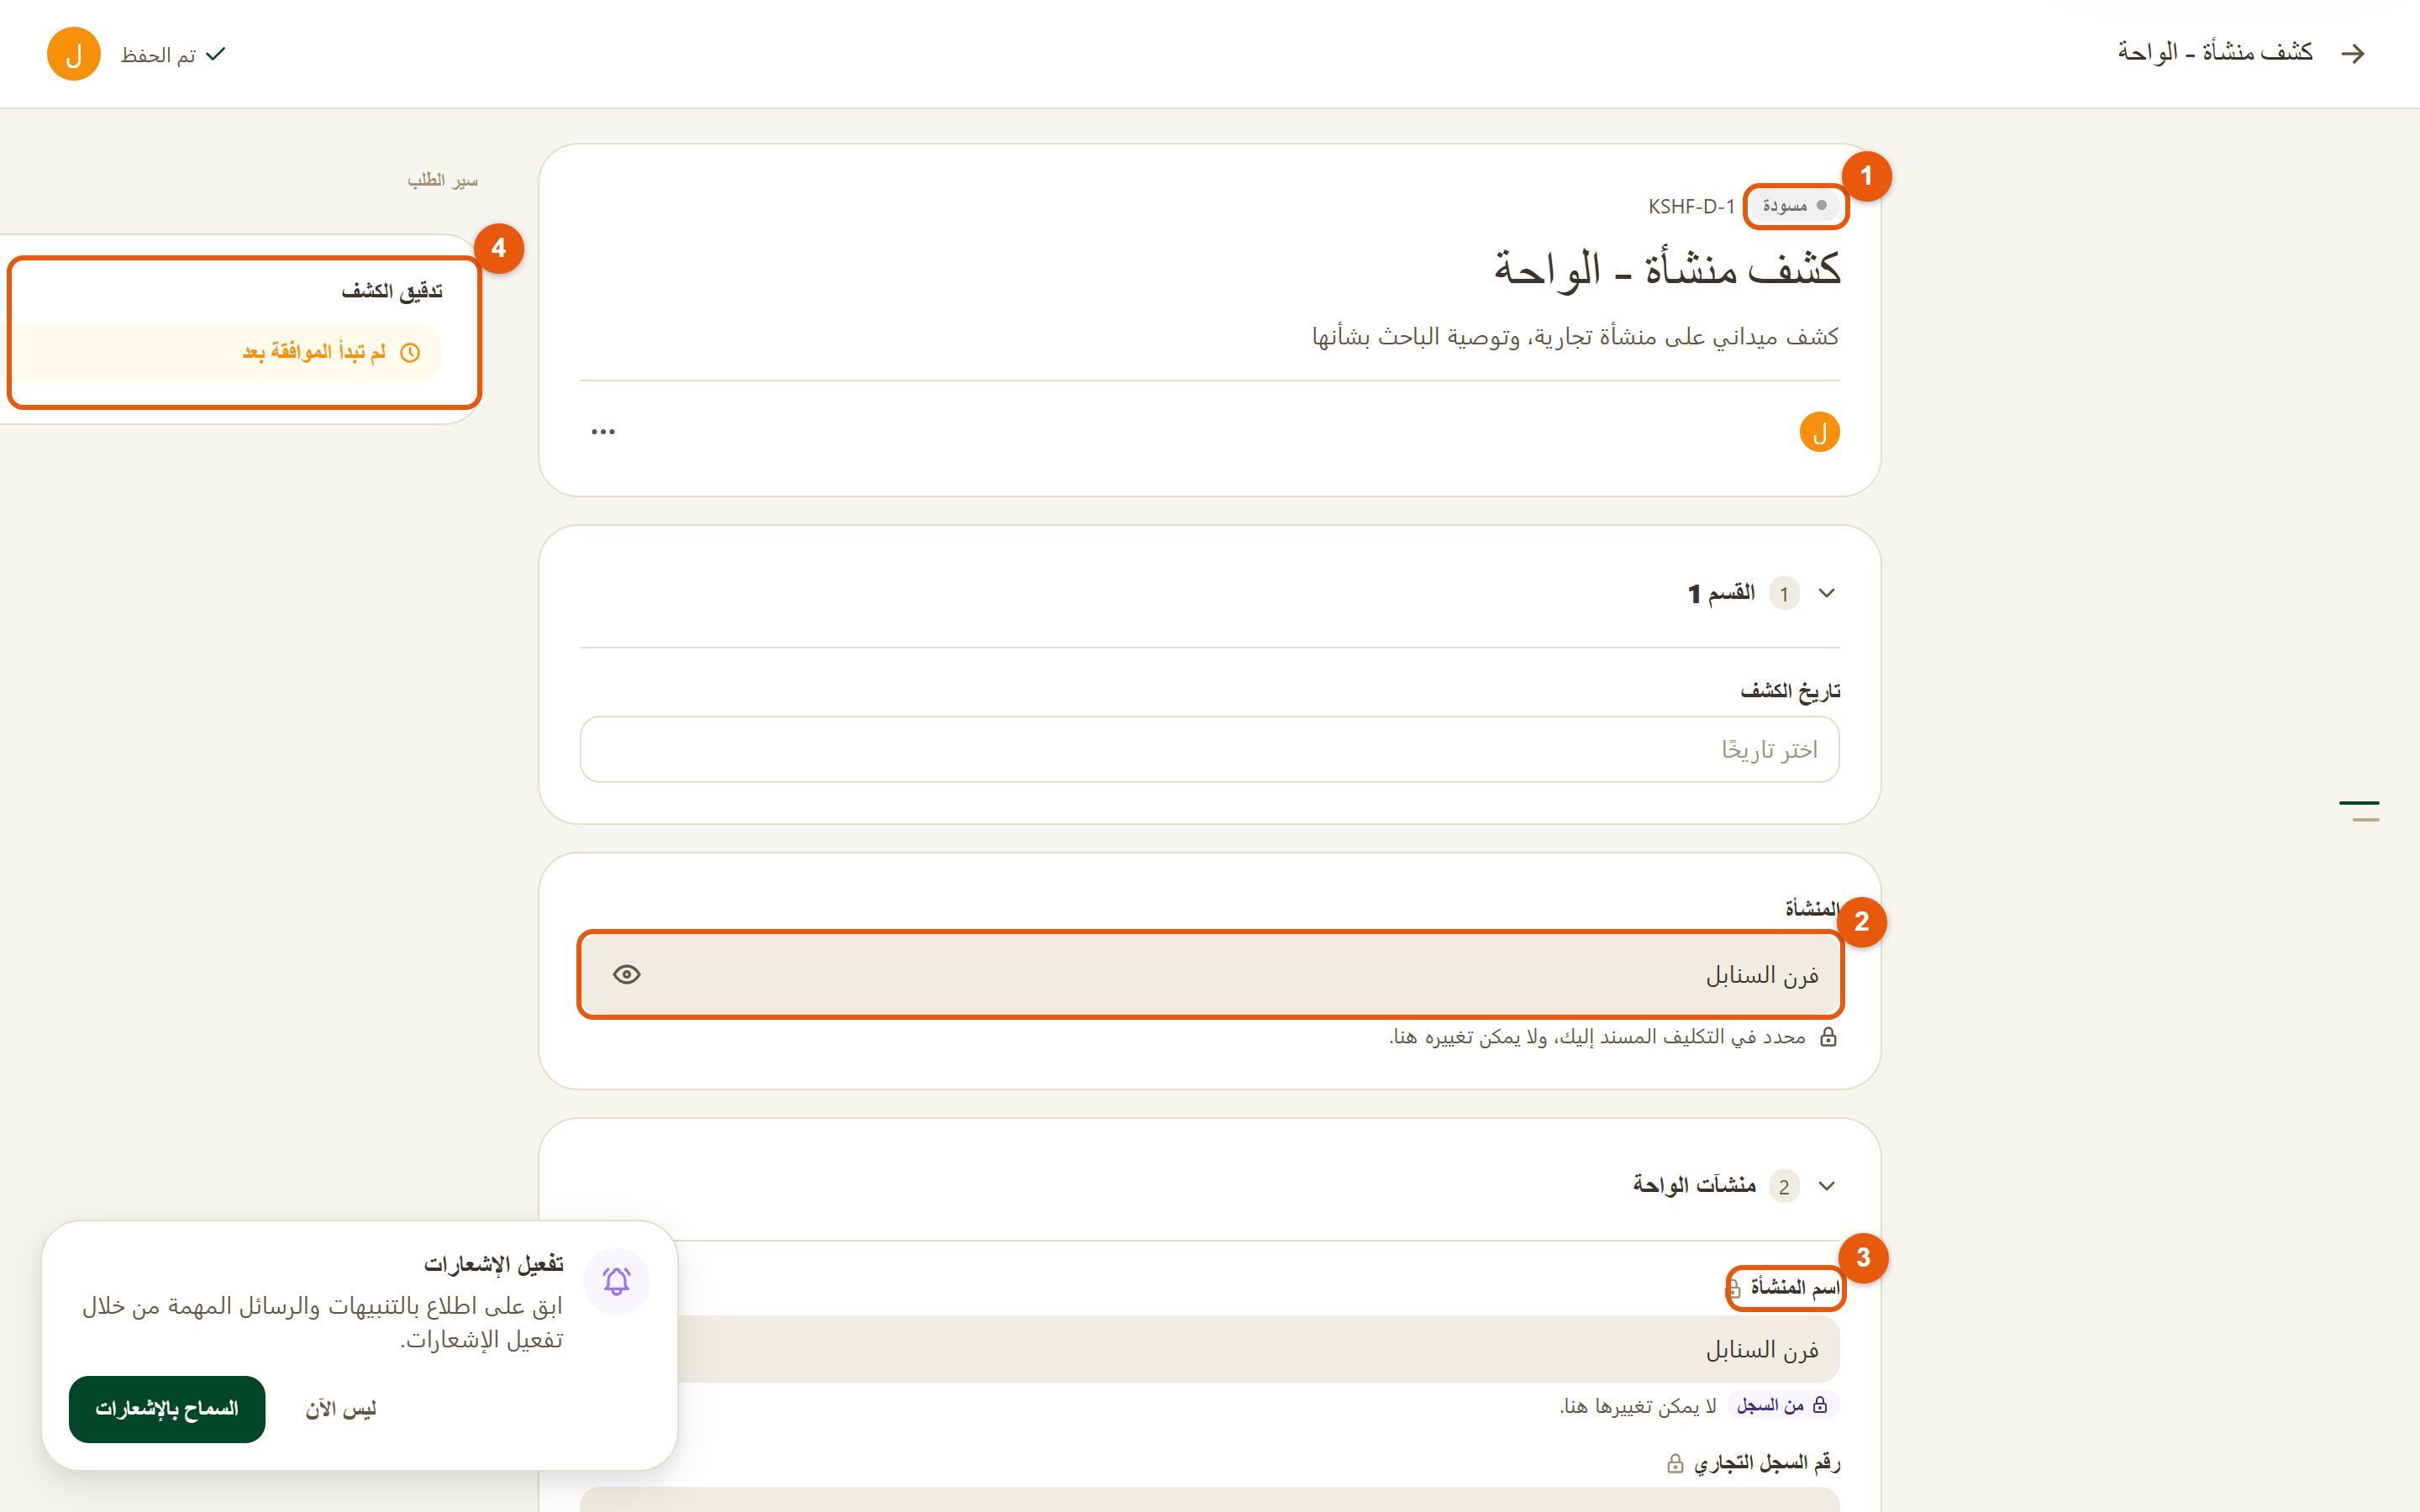
\includegraphics[width=0.95\linewidth]{assets/screens/b-laila-form.png}
\caption{الكشف كما يفتحه الباحث}
\label{fig:build-laila-form}
\shotnote{تأتي المنشأة من التكليف ولا يغيّرها الباحث. وتأتي بياناتها من سجلها، فيُقفل ما يُقرأ فقط. ① الحالة: «مسودة» حتى الإرسال. ② المنشأة: «محدد في التكليف المسند إليك». ③ حقل مقفل «من السجل». ④ «تدقيق الكشف» في انتظار الإرسال.}
\end{figure}

\subsection{خطوات العمل والتحقق}
\begin{enumerate}
\item اضغط «تكليفات مطلوبة منك»، ثم «ابدأ» بجانب المنشأة.
\item املأ الأسئلة. وإذا عدّلت حقلاً من السجل، يظهر تحته النص القديم مع «استعادة».
\item اضغط «إرسال الطلب»، ثم أكّد.
\end{enumerate}

\textbf{تحقق:} يجب أن تصبح الحالة «مُرسل» وأن يُقفل الكشف. وافتح المنشأة: يجب أن يبقى عنوانها القديم حتى الاعتماد.

\section{قرّر بحساب المدقق}
\label{sec:build-run-auditor}

يجد المدقق الكشف في «موافقات بانتظارك». ولا يستطيع القرار قبل أن يفتح كل الأقسام، ويطلب «رفض» و«إعادة للتصحيح» تعليقاً. ثم يقرّ بما راجعه، فيُحفظ القرار مع بصمة المحتوى.

\begin{rcnote}[مثال: مديرية الواحة]
اعتمدت رنا الكشف، فتحوّل إلى «مقبول»، وأصبح عنوان الفرن «المزة، شارع الجلاء، بناء 12» وحالته «موثقة». وفي كشف آخر أعادته للتصحيح، فظهرت ملاحظتها لليلى. ولما أُعيد إرساله رفضته، فبقيت المنشأة دون تغيير.
\end{rcnote}

\begin{figure}[H]
\centering
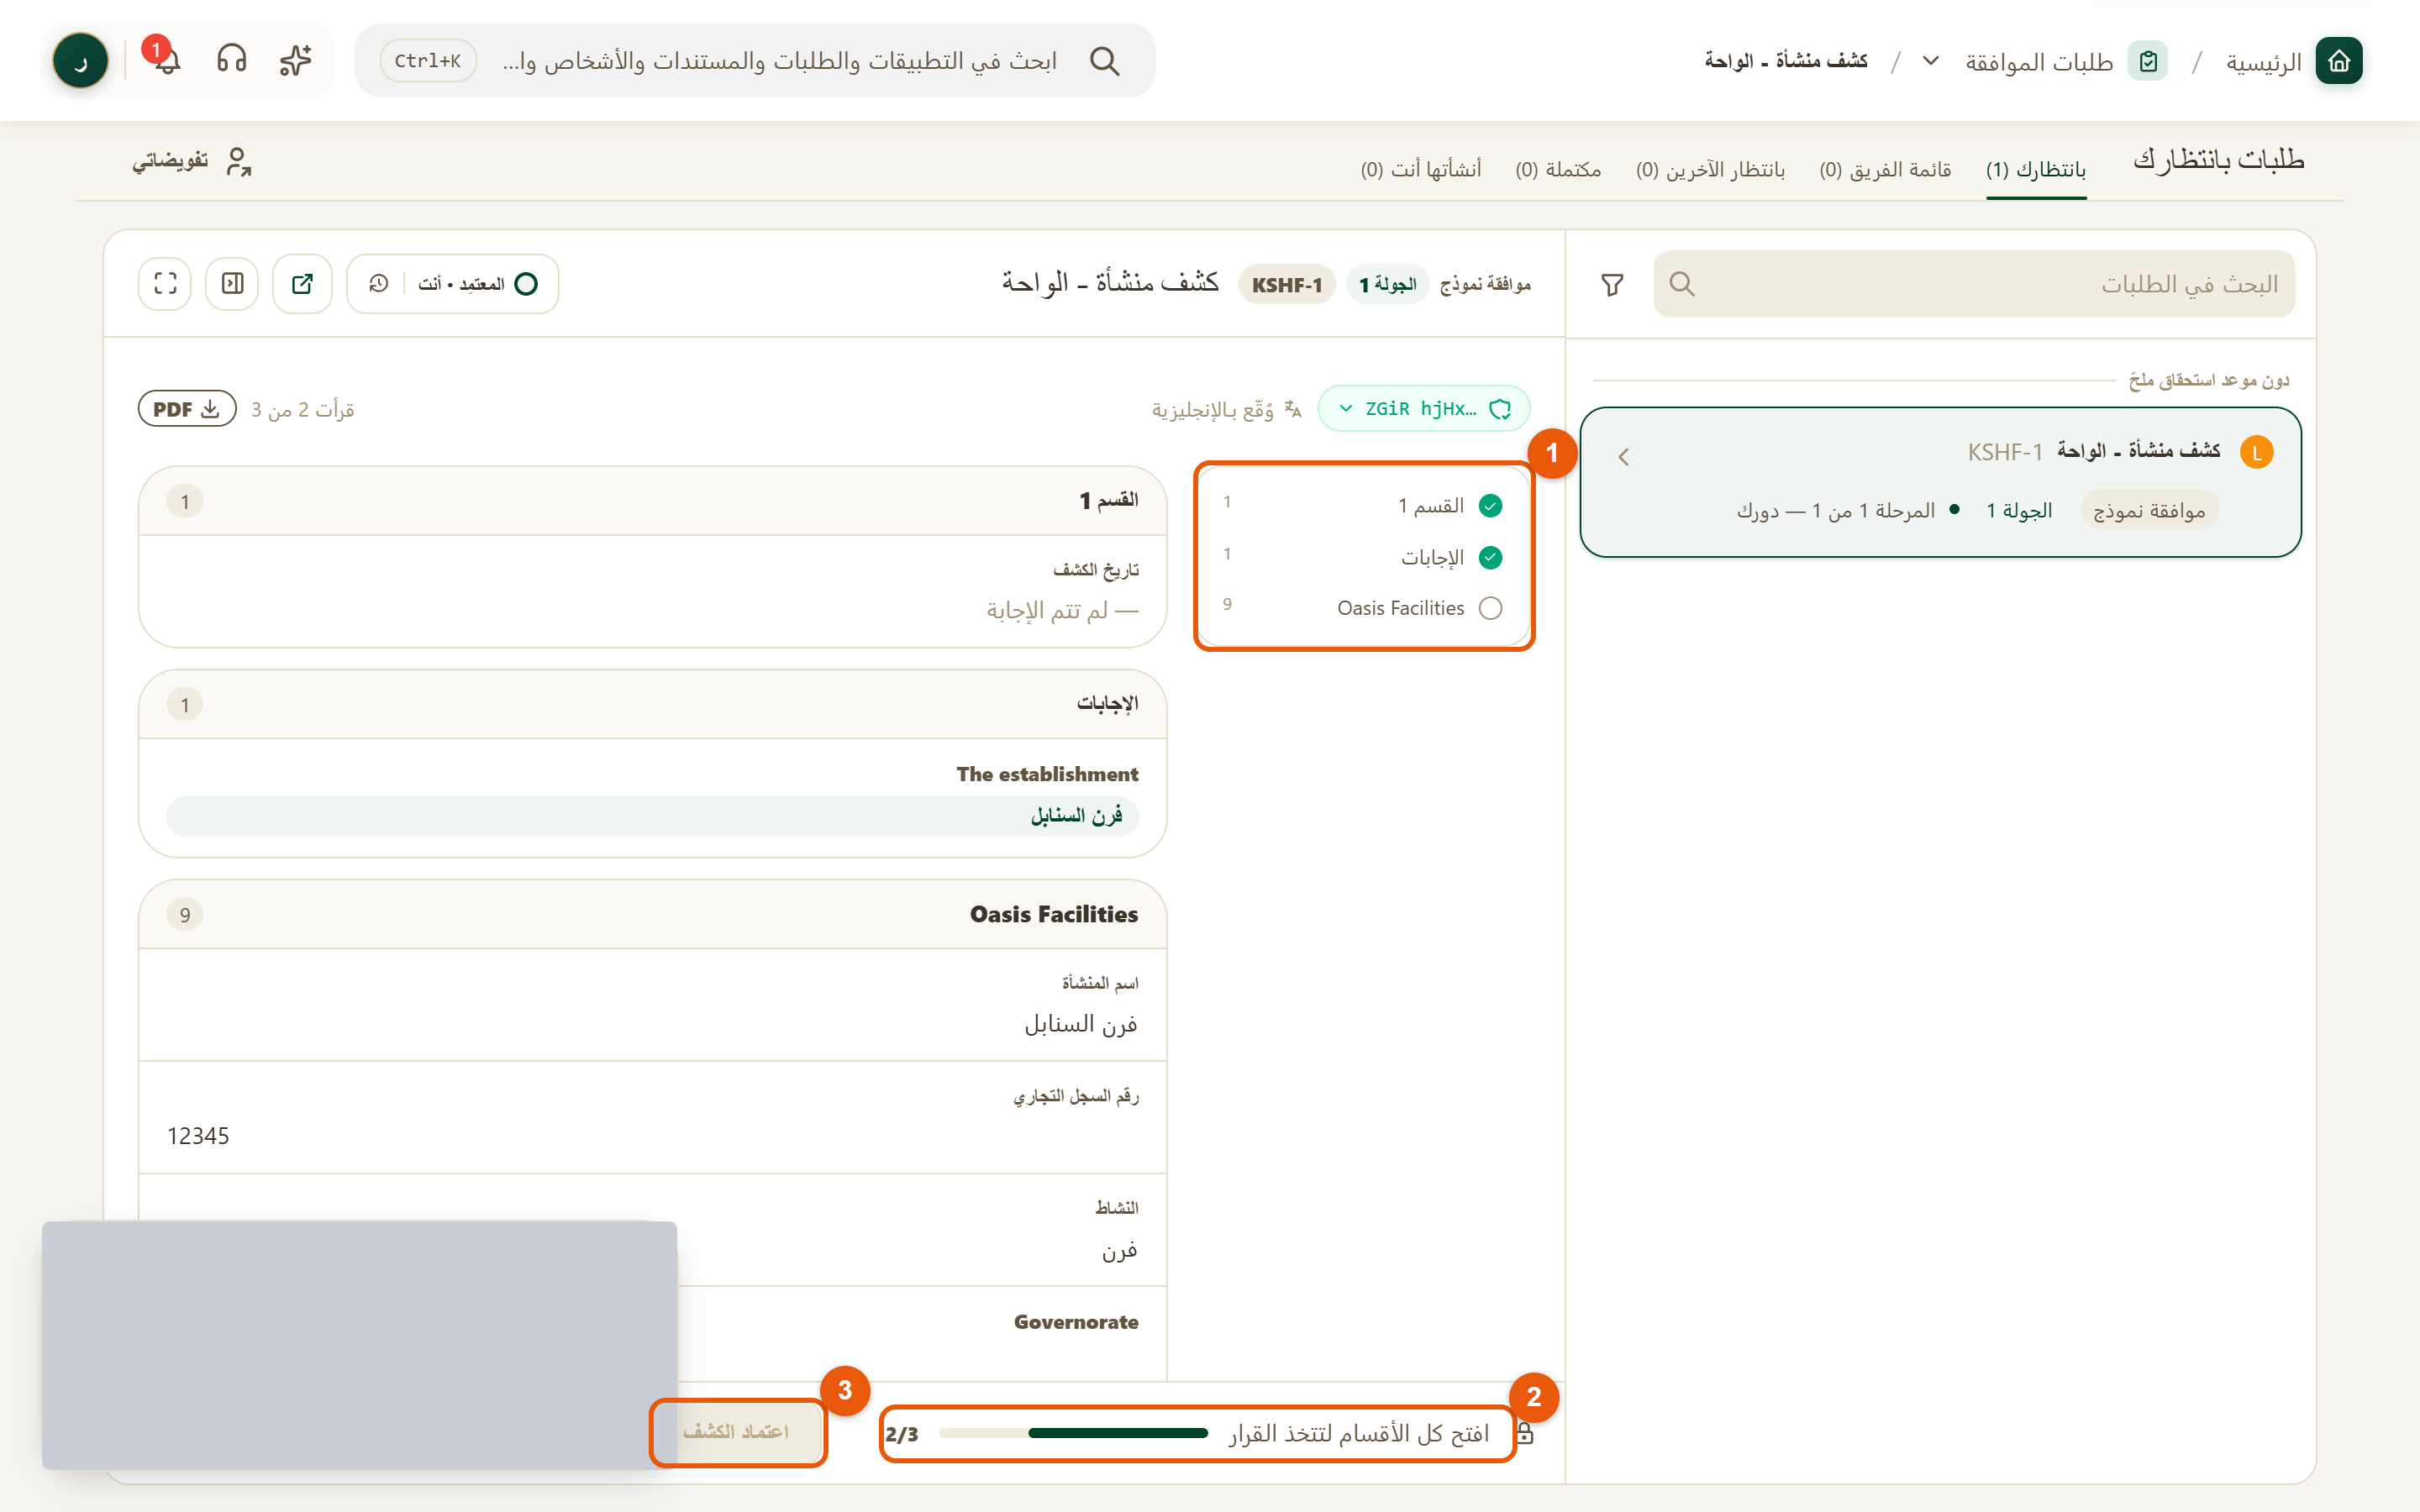
\includegraphics[width=0.95\linewidth]{assets/screens/b-decide.png}
\caption{شاشة قرار المدقق}
\label{fig:build-decide}
\shotnote{تعدّ الشاشة الأقسام المقروءة، ولا تفتح القرار قبل اكتمالها. ① الأقسام وما قُرئ منها. ② «افتح كل الأقسام لتتخذ القرار». ③ أزرار القرار.}
\end{figure}

\begin{figure}[H]
\centering
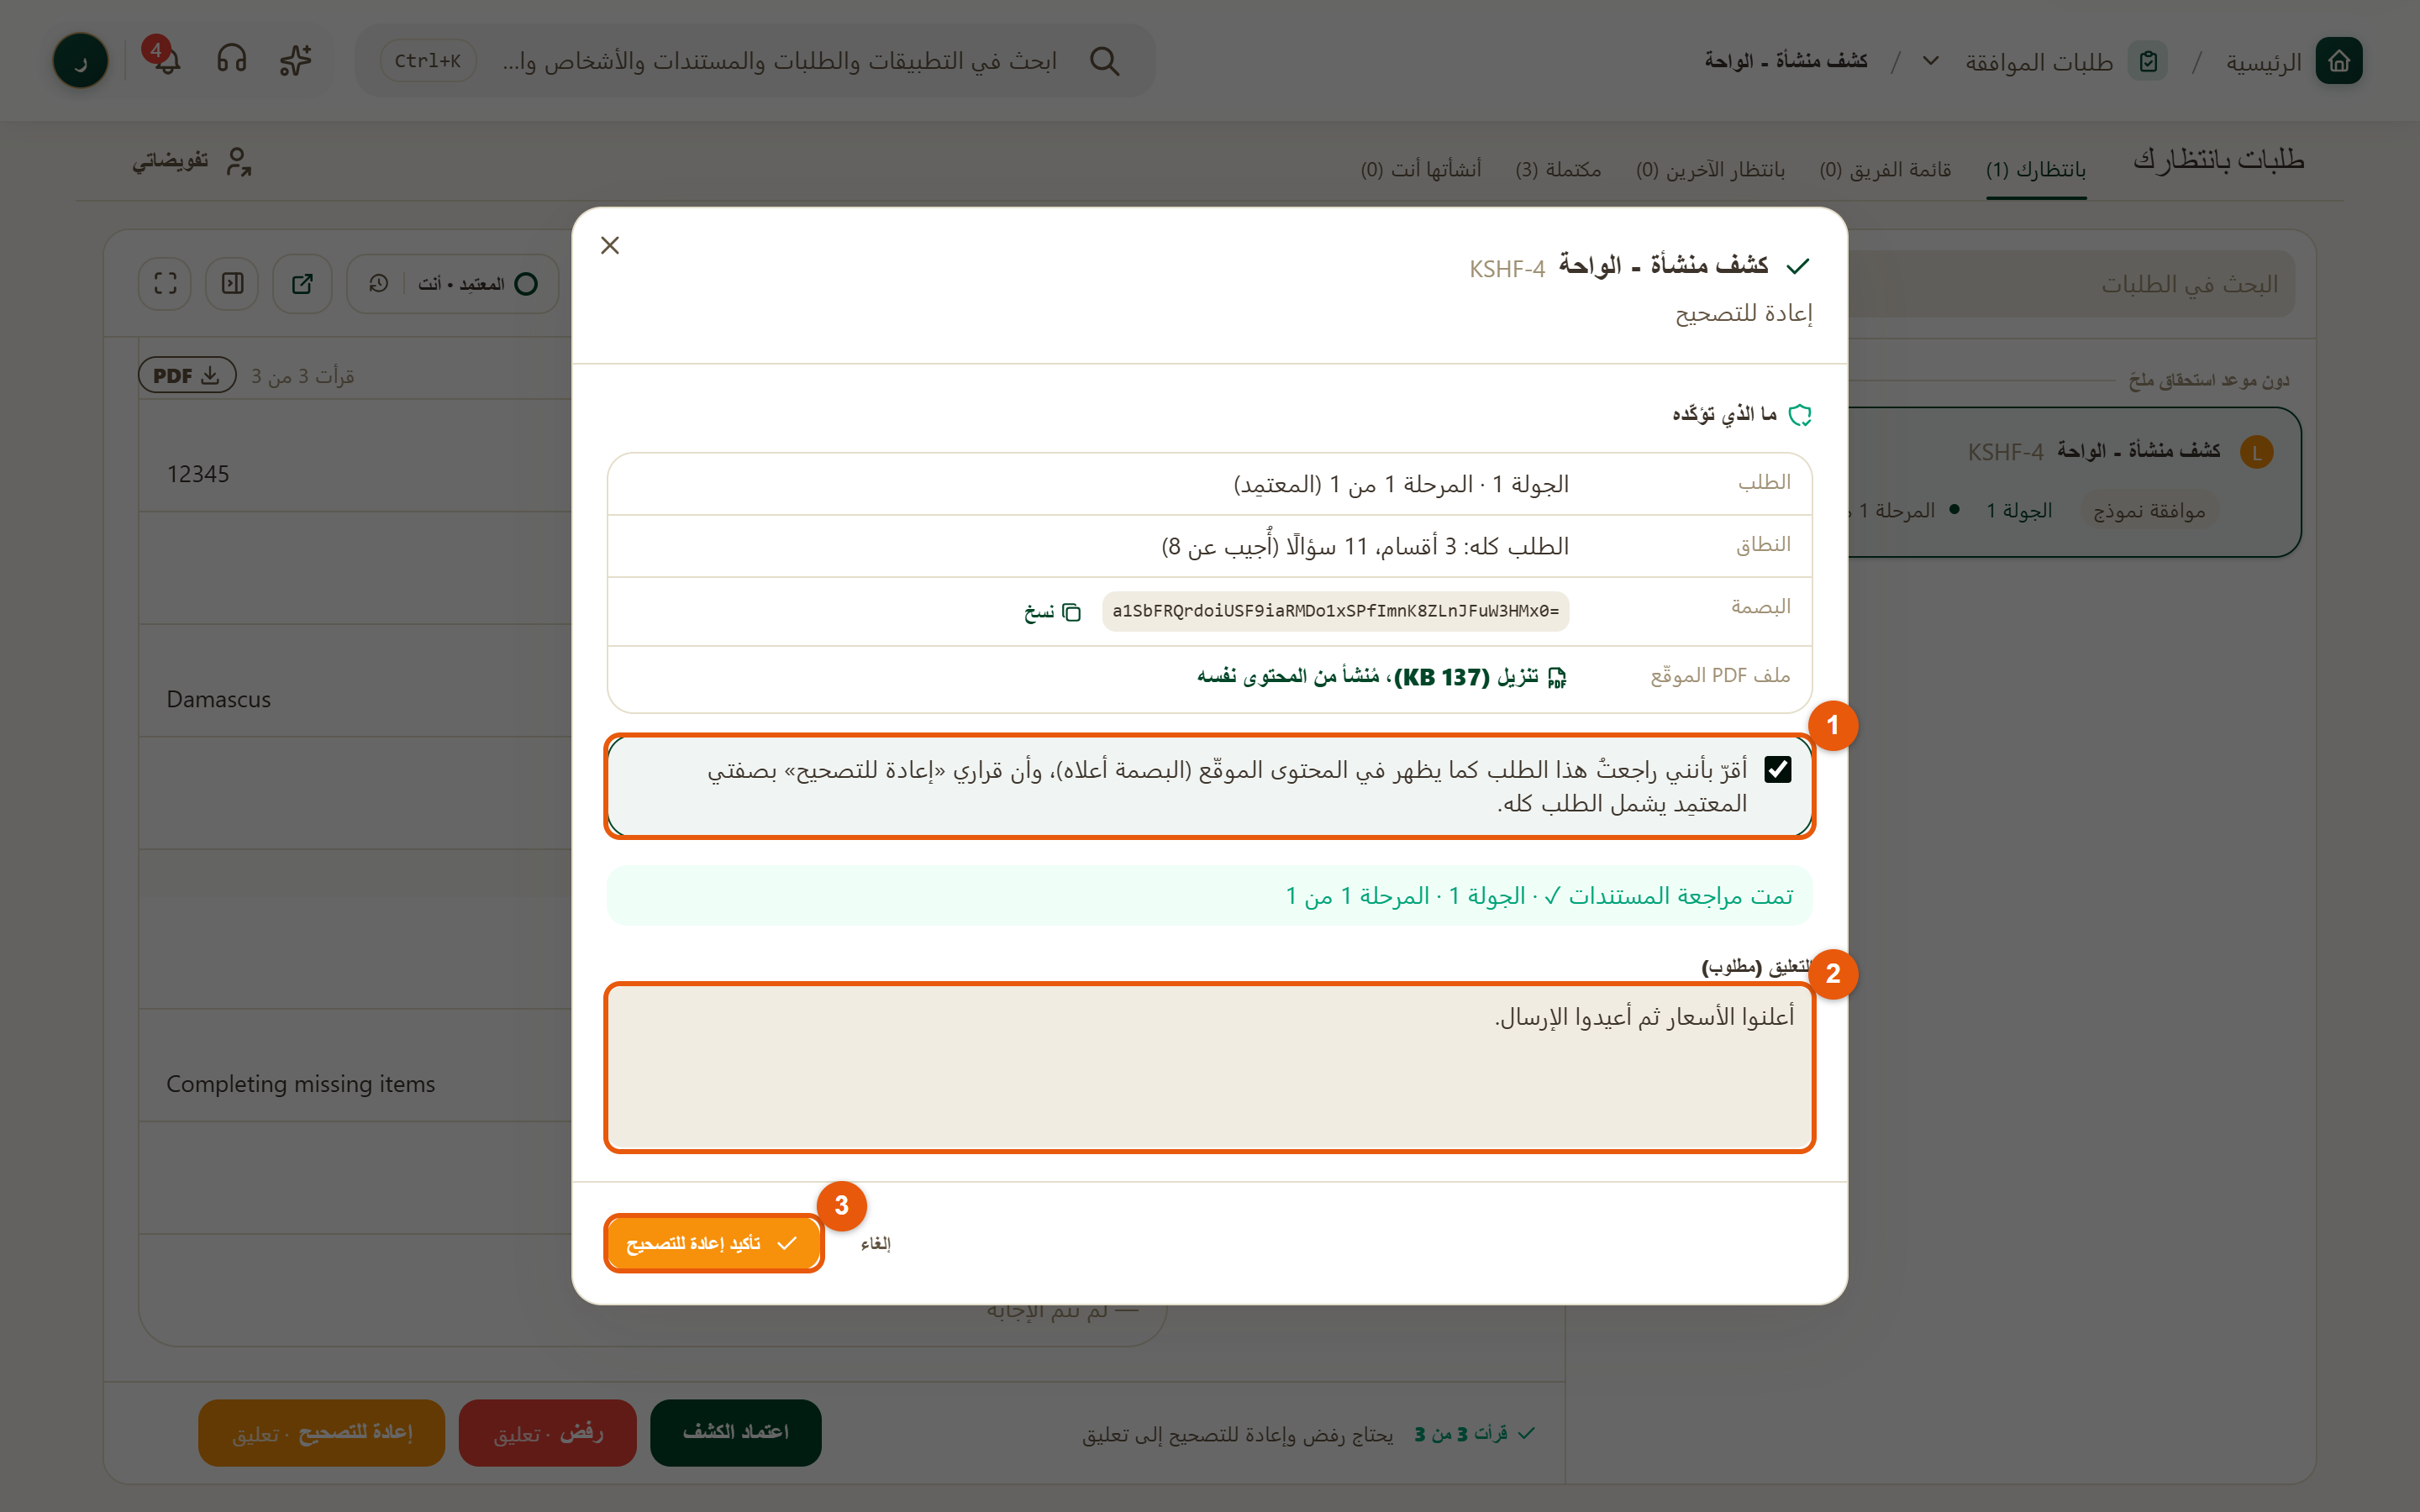
\includegraphics[width=0.95\linewidth]{assets/screens/b-return-dlg.png}
\caption{تأكيد القرار}
\label{fig:build-return-dlg}
\shotnote{يلخّص التأكيد ما يقرّ به المدقق، ومعه بصمة المحتوى وملف PDF موقّع. ① الإقرار: لا يُقبل القرار دونه. ② «التعليق (مطلوب)» للرفض والإعادة. ③ زر التأكيد.}
\end{figure}

\begin{figure}[H]
\centering
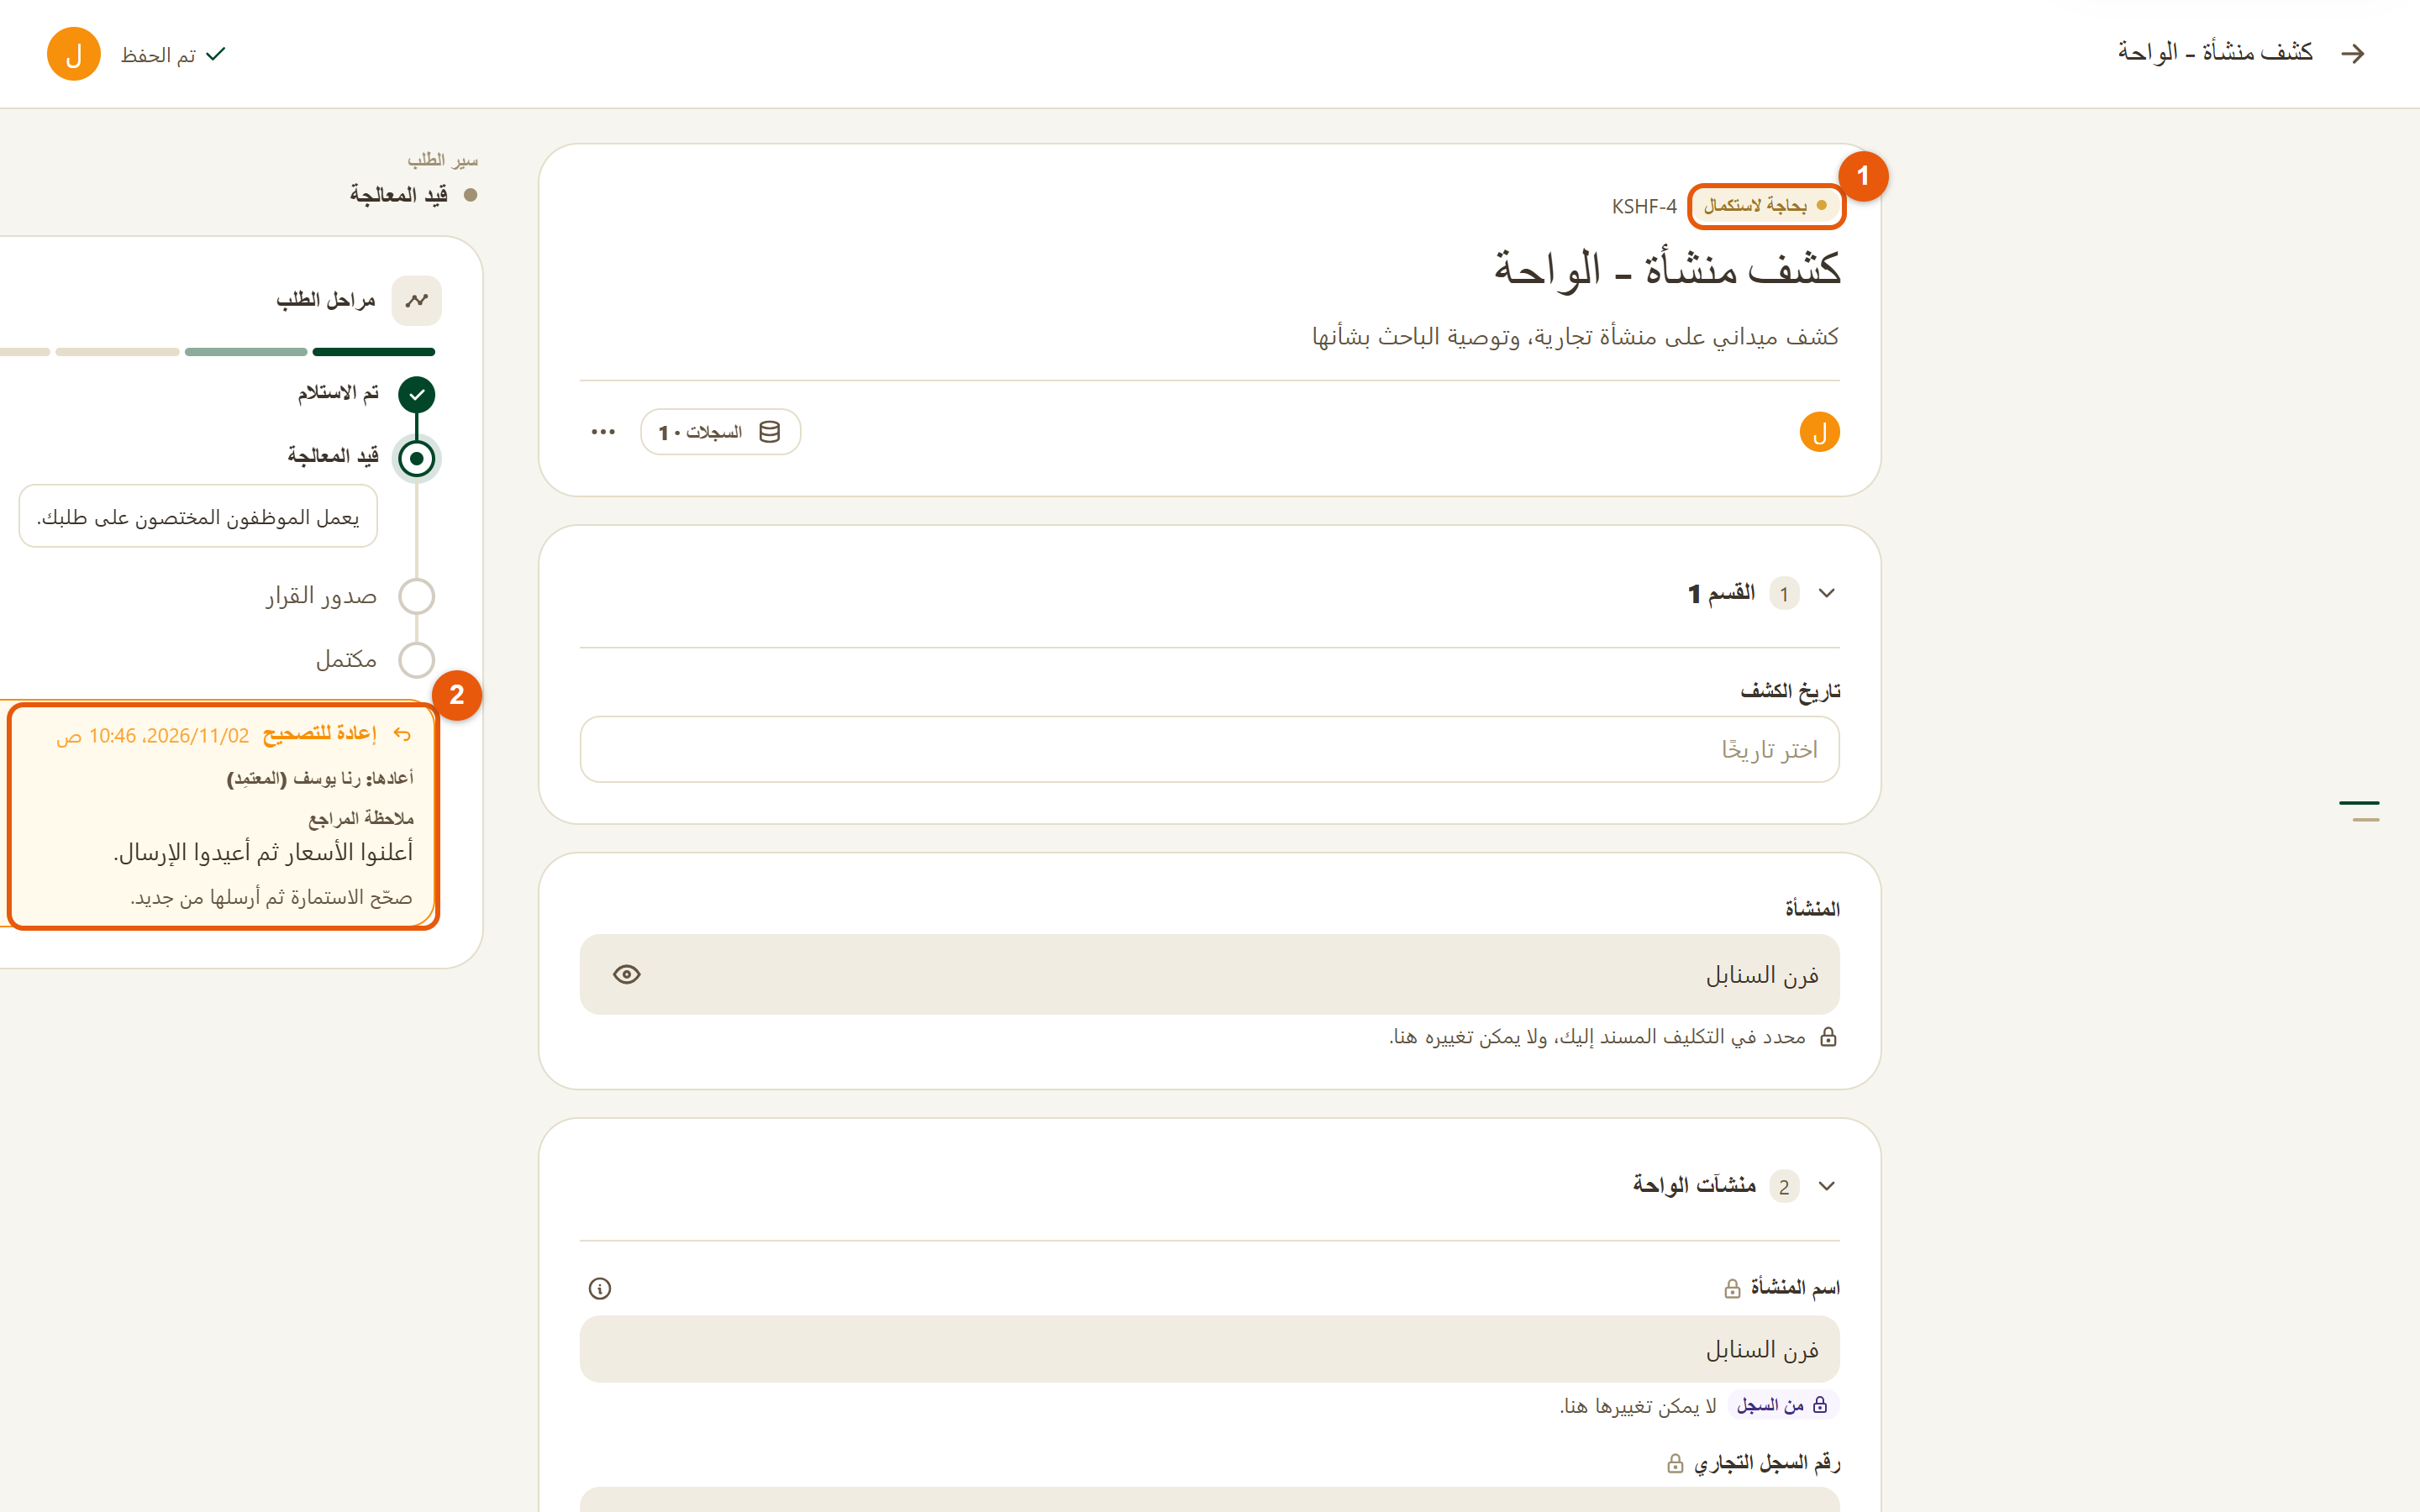
\includegraphics[width=0.95\linewidth]{assets/screens/b-returned.png}
\caption{ما يراه الباحث بعد الإعادة}
\label{fig:build-returned}
\shotnote{يعود الكشف قابلاً للتعديل، ومعه ملاحظة المدقق. وإعادة إرساله تبدأ جولة موافقة جديدة. ① «بحاجة لاستكمال». ② «إعادة للتصحيح» مع اسم المدقق وملاحظته.}
\end{figure}

\begin{figure}[H]
\centering
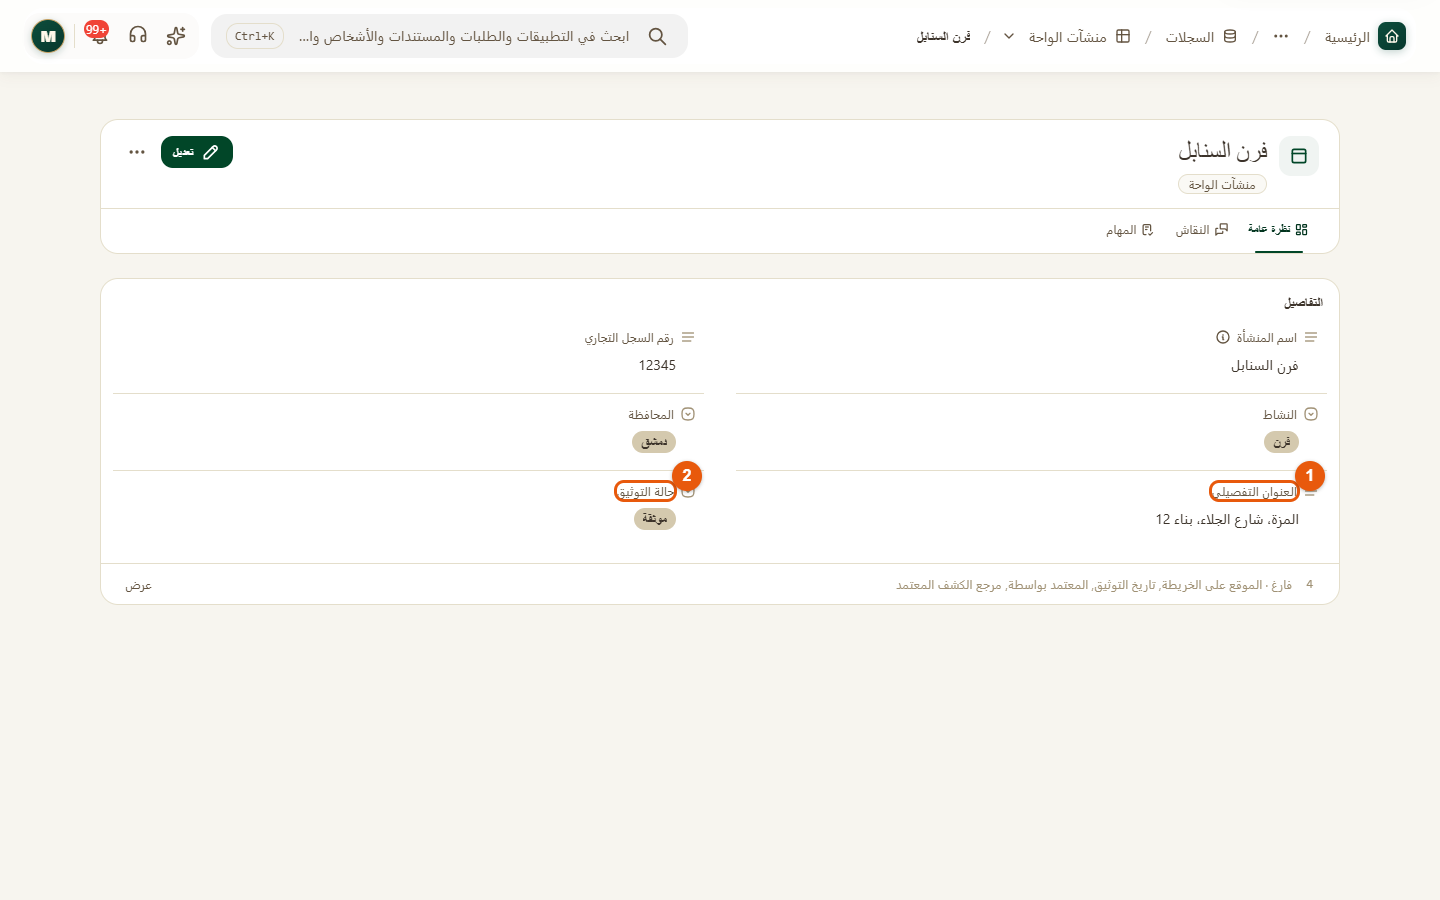
\includegraphics[width=0.95\linewidth]{assets/screens/b-record-after.png}
\caption{المنشأة بعد الاعتماد}
\label{fig:build-record-after}
\shotnote{هذه نتيجة السيناريو كله: لم يحدّث سجل المنشأة إلا الكشف المعتمد. ① «العنوان التفصيلي» الجديد. ② «حالة التوثيق»: «موثقة».}
\end{figure}

\subsection{خطوات العمل والتحقق}
\begin{enumerate}
\item افتح «موافقات بانتظارك»، ثم الكشف.
\item افتح كل قسم من القائمة الجانبية، ومرّر حتى نهايته، حتى يصبح العدّاد «قرأت 3 من 3».
\item اضغط القرار، واكتب التعليق إن طُلب، وحدّد الإقرار، ثم اضغط «تأكيد».
\end{enumerate}

\textbf{تحقق:} افتح المنشأة بعد الاعتماد، ويجب أن تحمل القيم الجديدة. وإذا ظهر في الكشف «تمت الموافقة — تعذّر تطبيق التغييرات»، فانتقل إلى القسم التالي.

\section{أضف نوع سجلات «المنشآت الصناعية»}
\label{sec:build-industrial}

تحتاج لوحة المؤشرات إلى بيانات تقرؤها. لذلك تبدأ بنوع سجلات يحفظ ما تريد قياسه: عدداً تعدّه، أو رقماً تجمعه، أو خياراً توزّع عليه. ويُبنى بالطريقة نفسها التي بُني بها «منشآت الواحة».

\begin{rcnote}[مثال: مديرية الواحة]
تتابع المديرية عشر منشآت صناعية في محافظات مختلفة. وتريد أن تعرف عددها، ومجموع عمالها، وطاقتها الإنتاجية، وتوزّعها حسب المحافظة والقطاع وحالة الترخيص.
\end{rcnote}

\begin{table}[H]
\centering
\caption{حقول «المنشآت الصناعية» ودورها في اللوحة}
\label{tab:build-industrial-fields}
\begin{tabularx}{\linewidth}{R{3.8cm} R{2.2cm} Y}
\rcHeaderRow
\thh{الحقل} & \thh{النوع} & \thh{ما يتيحه في اللوحة}\\
اسم المنشأة & نص & اسم يظهر في الجداول.\\
القطاع & اختيار & غذائية، نسيجية، كيميائية، هندسية؛ للتوزيع حسب القطاع.\\
المحافظة & اختيار & المحافظات الأربع عشرة؛ للتوزيع حسب المحافظة.\\
عدد العمال & رقم & يُجمع ويُحسب متوسطه.\\
الطاقة الإنتاجية بالطن & رقم & يُجمع ويُحسب متوسطه.\\
حالة الترخيص & اختيار & مرخصة، قيد الترخيص، موقوفة.\\
تاريخ آخر كشف & تاريخ & للتصفية حسب الفترة.\\
\end{tabularx}
\end{table}

\begin{figure}[H]
\centering
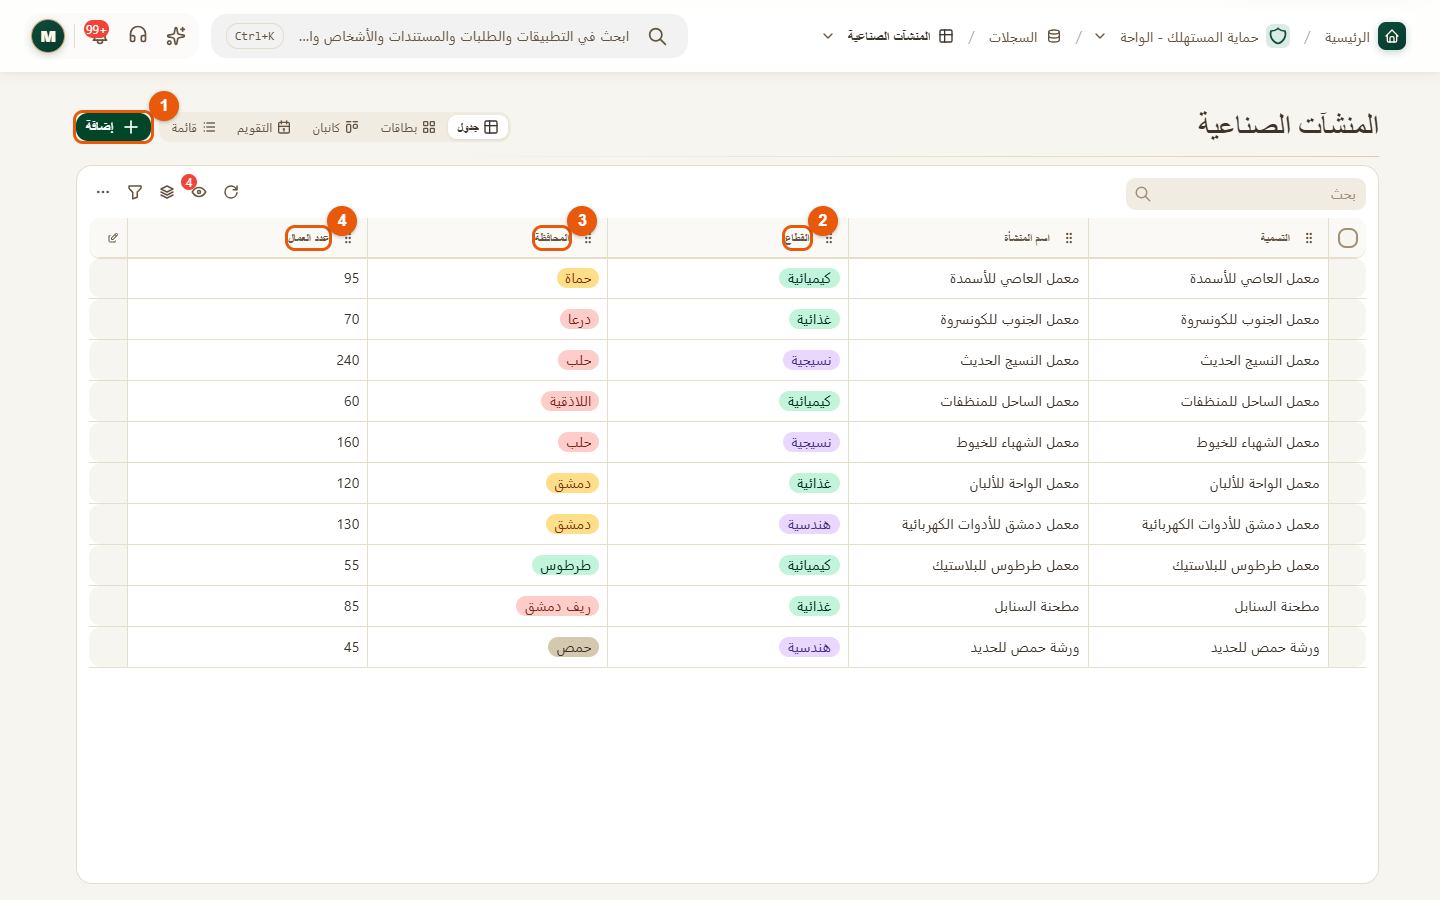
\includegraphics[width=0.95\linewidth]{assets/screens/i-records.png}
\caption{سجلات المنشآت الصناعية}
\label{fig:build-industrial-records}
\shotnote{هذه البيانات التي ستقرؤها اللوحة، وتقابلها كل أرقامها. فإذا اختلف رقم في اللوحة عما تعدّه هنا يدوياً، فراجع إعداد العنصر. ① «إضافة»: يضيف منشأة. ② «القطاع». ③ «المحافظة». ④ «عدد العمال».}
\end{figure}

\subsection{خطوات العمل والتحقق}
\begin{enumerate}
\item افتح «الكيانات» ← «إضافة كيان»، وأضف الحقول بحسب الجدول، كما في قسم «أنشئ التطبيق ونوع السجلات».
\item اختر في «إعدادات الكيان» «اسم المنشأة» للاسم المعروض، وفعّل «إظهار في التنقل»، واختر التطبيق والقسم، ثم اضغط «انشاء كيان».
\item أدخل السجلات من «سجل جديد» في التطبيق.
\end{enumerate}

\textbf{تحقق:} افتح نوع السجلات في التطبيق، ويجب أن يظهر عدد السجلات بجانب اسمه.

\section{أنشئ لوحة المؤشرات}
\label{sec:build-dashboard}

اللوحة صفحة تجمع عناصر، وكل عنصر يقرأ نوع سجلات ويعرض منه رقماً أو رسماً أو جدولاً. حدّد قبل البناء الأسئلة التي يجب أن تجيب عنها، ثم اختر لكل سؤال عنصراً.

\begin{rcnote}[مثال: مديرية الواحة]
أنشأت المديرية لوحة «مؤشرات المنشآت الصناعية - الواحة»، وحددت ثمانية أسئلة لها، كما في الجدول التالي.
\end{rcnote}

\begin{table}[H]
\centering
\caption{الأسئلة وعناصرها}
\label{tab:build-dashboard-plan}
\begin{tabularx}{\linewidth}{Y R{3cm} R{3.6cm}}
\rcHeaderRow
\thh{السؤال} & \thh{العنصر} & \thh{النتيجة في المثال}\\
كم منشأة نتابع؟ & مؤشر أداء: العدد & 10\\
كم عاملاً فيها؟ & مؤشر أداء: المجموع & 1060\\
ما طاقتها الإنتاجية؟ & مؤشر أداء: المجموع & 36600 طن\\
كم منشأة موقوفة؟ & مؤشر أداء بتصفية & 2\\
أين تقع؟ & رسم أعمدة: عدد & حلب ودمشق 2، والبقية 1\\
ما قطاعاتها؟ & رسم دائري & 30\% غذائية، 30\% كيميائية، 20\% لكل من النسيجية والهندسية\\
أين يعمل أكثر العمال؟ & رسم أعمدة: مجموع & نسيجية 400، غذائية 275، كيميائية 210، هندسية 175\\
ما حالة تراخيصها؟ & رسم دائري & 60\% مرخصة، 20\% قيد الترخيص، 20\% موقوفة\\
\end{tabularx}
\end{table}

\begin{figure}[H]
\centering
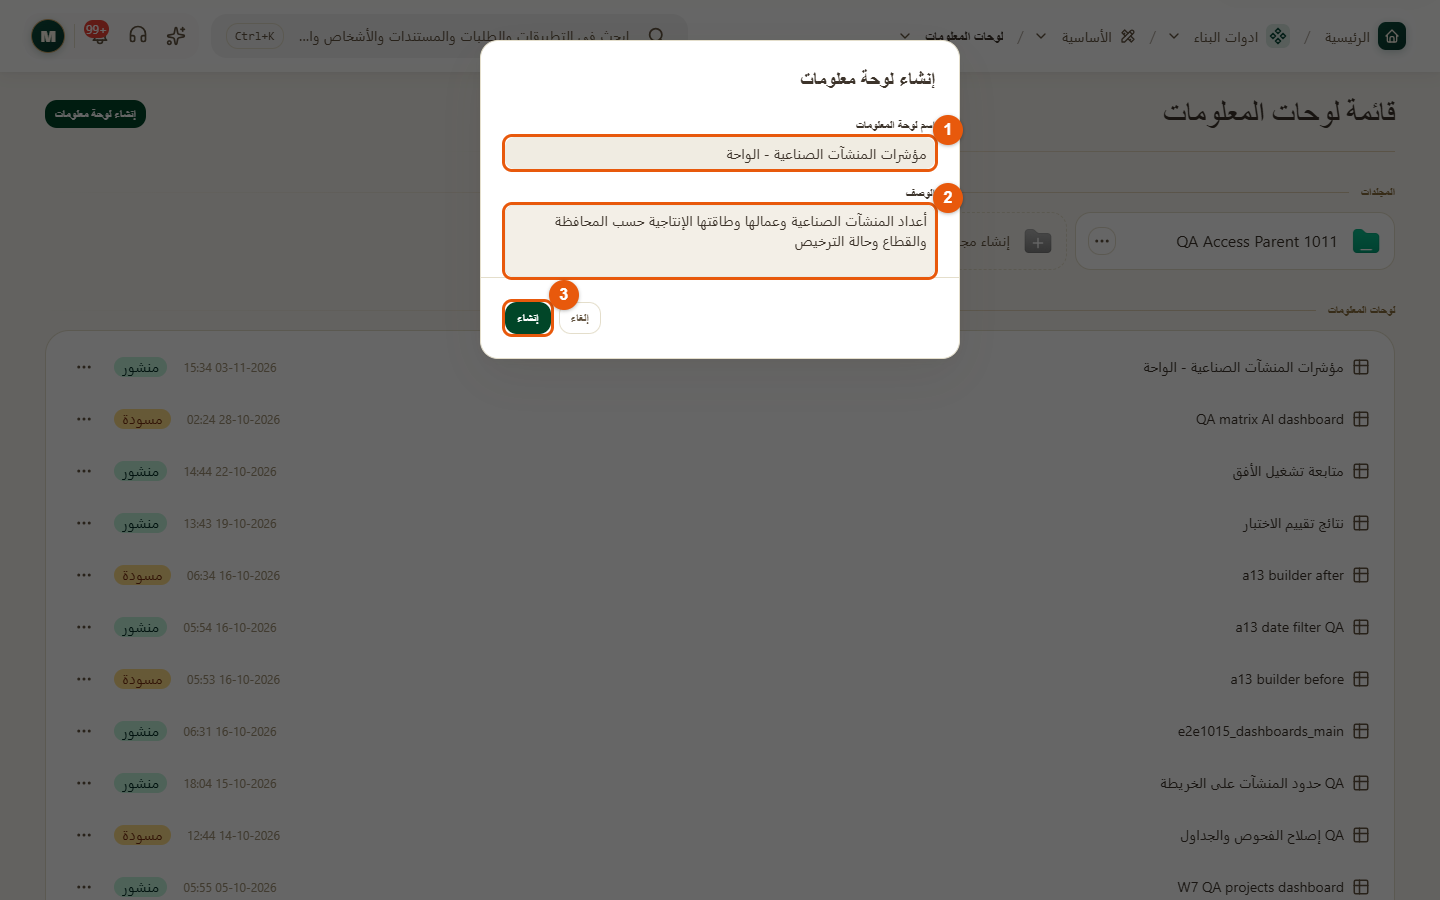
\includegraphics[width=0.62\linewidth]{assets/screens/i-new.png}
\caption{إنشاء لوحة معلومات}
\label{fig:build-dashboard-new}
\shotnote{تطلب النافذة الاسم والوصف فقط، ثم تفتح محرر اللوحة مباشرة. ① «اسم لوحة المعلومات». ② «الوصف»: يظهر تحت الاسم لمن يفتح اللوحة. ③ «إنشاء».}
\end{figure}

\begin{figure}[H]
\centering
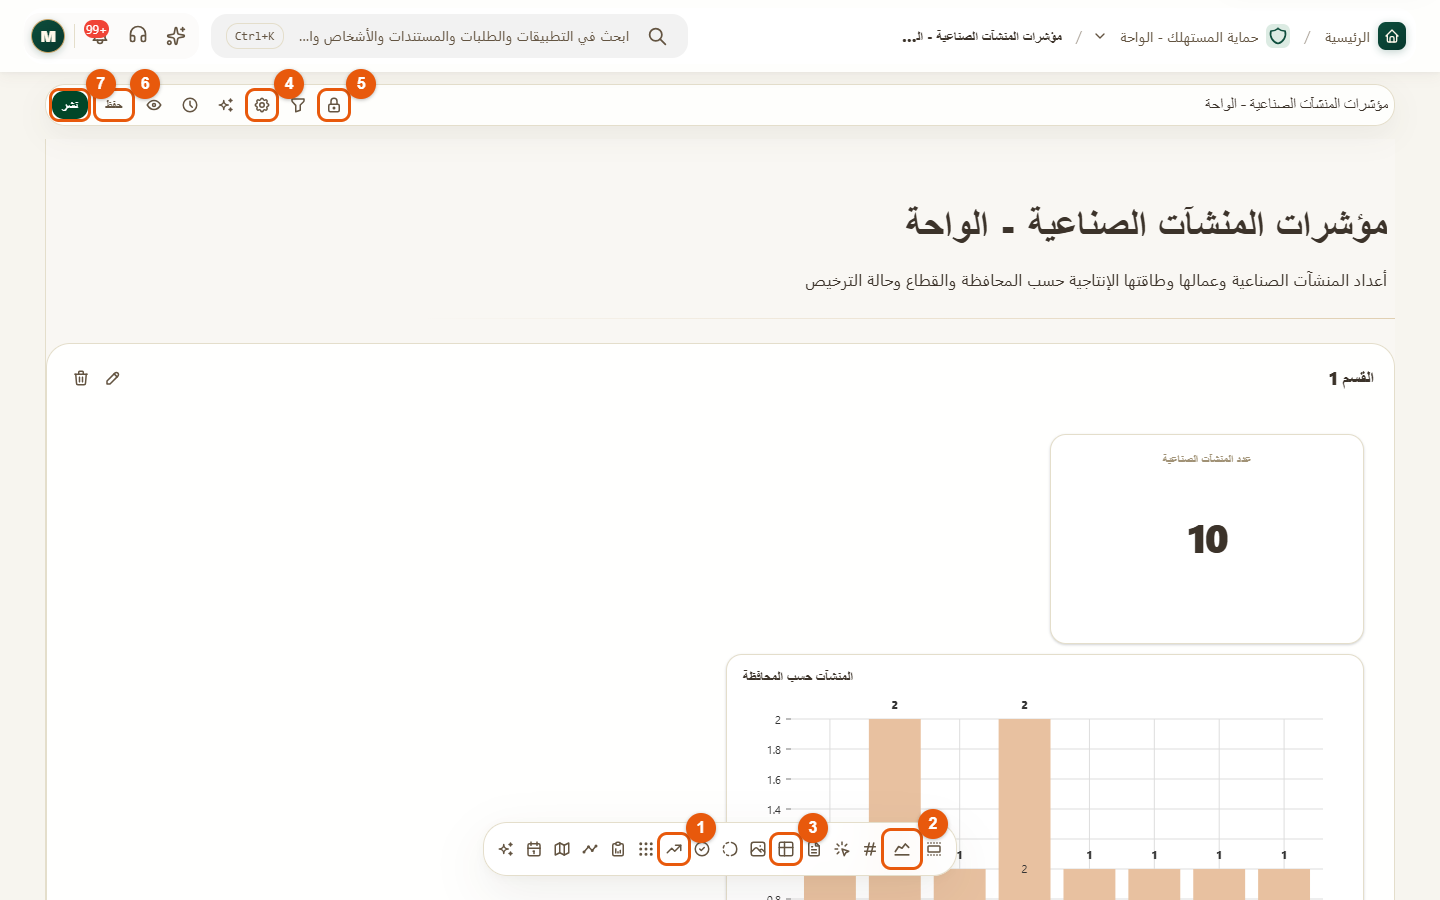
\includegraphics[width=0.95\linewidth]{assets/screens/i-builder.png}
\caption{محرر اللوحة}
\label{fig:build-dashboard-builder}
\shotnote{يضيف الشريط السفلي العناصر، ويضبط الشريط العلوي اللوحة كلها. ① «مؤشر أداء»: رقم واحد. ② «إضافة رسم بياني (Nivo)»: أعمدة أو دائري وغيرهما. ③ «جدول». ④ «الإعدادات»: الاسم والتطبيق والقسم. ⑤ «إدارة الوصول»: من يرى اللوحة. ⑥ «حفظ». ⑦ «نشر»: لا يرى المشاهدون أي تعديل قبله.}
\end{figure}

\subsection{خطوات العمل والتحقق}
\begin{enumerate}
\item افتح «ادوات البناء» ← «لوحات المعلومات» ← «إنشاء لوحة معلومات».
\item اكتب الاسم والوصف، ثم اضغط «إنشاء».
\end{enumerate}

\textbf{تحقق:} يجب أن يفتح المحرر وفيه «القسم 1» فارغاً.

\section{اربط المؤشرات بنوع السجلات}
\label{sec:build-kpi}

يبدأ كل عنصر بلا بيانات، أو ببيانات تجريبية. وتربطه بنوع السجلات من تبويب «البيانات»: تختار «كيان» مصدراً، ثم نوع السجلات، ثم طريقة الحساب. وتحسب «العدد» عدد السجلات، أما «المجموع» و«المتوسط» فتحتاج إلى حقل رقمي.

\begin{rcnote}[مثال: مديرية الواحة]
مؤشر «إجمالي العمال» يجمع «عدد العمال» من «المنشآت الصناعية»، فيعطي 1060. ومؤشر «عدد المنشآت الصناعية» يستخدم «العدد» دون حقل، فيعطي 10.
\end{rcnote}

\begin{figure}[H]
\centering
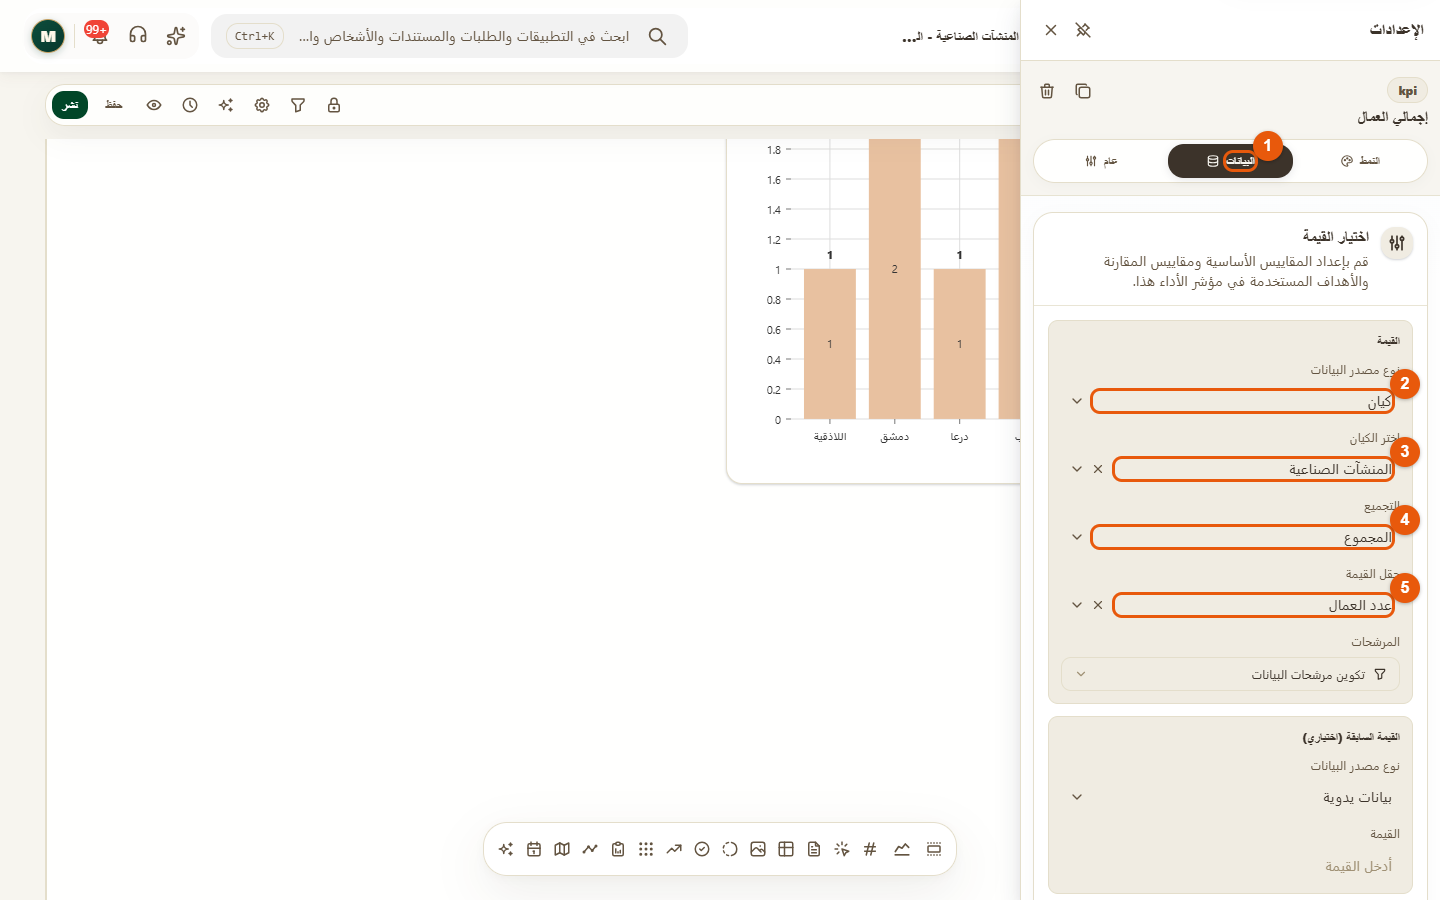
\includegraphics[width=0.95\linewidth]{assets/screens/i-kpi.png}
\caption{مصدر بيانات مؤشر الأداء}
\label{fig:build-kpi}
\shotnote{يعيد العنصر حساب رقمه فور تغيير أي إعداد، فترى النتيجة قبل الحفظ. ① «البيانات». ② «نوع مصدر البيانات»: «كيان». ③ «اختر الكيان». ④ «التجميع»: «العدد» أو «المجموع» أو «المتوسط» أو الحد الأدنى أو الأقصى. ⑤ «حقل القيمة»: الحقل الرقمي الذي يُجمع.}
\end{figure}

\subsection{خطوات العمل والتحقق}
\begin{enumerate}
\item اضغط «مؤشر أداء» في الشريط السفلي، فيُضاف العنصر وتُفتح إعداداته.
\item في «البيانات» ← «القيمة»: اختر «كيان»، ثم نوع السجلات، ثم «التجميع»، ثم «حقل القيمة» إن لزم.
\item افتح «عام»، واكتب «العنوان»، واضبط «العرض» و«الارتفاع». فالعرض 3 والارتفاع 2 يناسبان المؤشر.
\item أغلق الإعدادات، واضغط «حفظ».
\end{enumerate}

\textbf{تحقق:} قارن الرقم بالقائمة. وإذا ظهر «ليس لديك صلاحية لعرض هذه البيانات»، فقد اخترت نوع سجلات آخر يحمل الاسم نفسه؛ فافتح القائمة واختر الآخر، أو أعطِ نوع سجلاتك اسماً لا يتكرر.

\section{أضف الرسوم البيانية والجدول}
\label{sec:build-charts}

يوزّع الرسم السجلات على قيم حقل اختيار، مثل المحافظة. ويحدد «نوع القيمة» ما يرسمه لكل قيمة: «عدد» السجلات، أو «قيمة» حقل رقمي مع «التجميع». أما الرسم الدائري فيعدّ وحده، ولا يطلب إلا «حقل الفئة».

\begin{rcnote}[مثال: مديرية الواحة]
رسم «العمال حسب القطاع» أعمدة: فئته «القطاع»، ونوع قيمته «قيمة»، وحقل قيمته «عدد العمال»، وتجميعه «المجموع». فيُظهر 400 عامل في القطاع النسيجي.
\end{rcnote}

\begin{figure}[H]
\centering
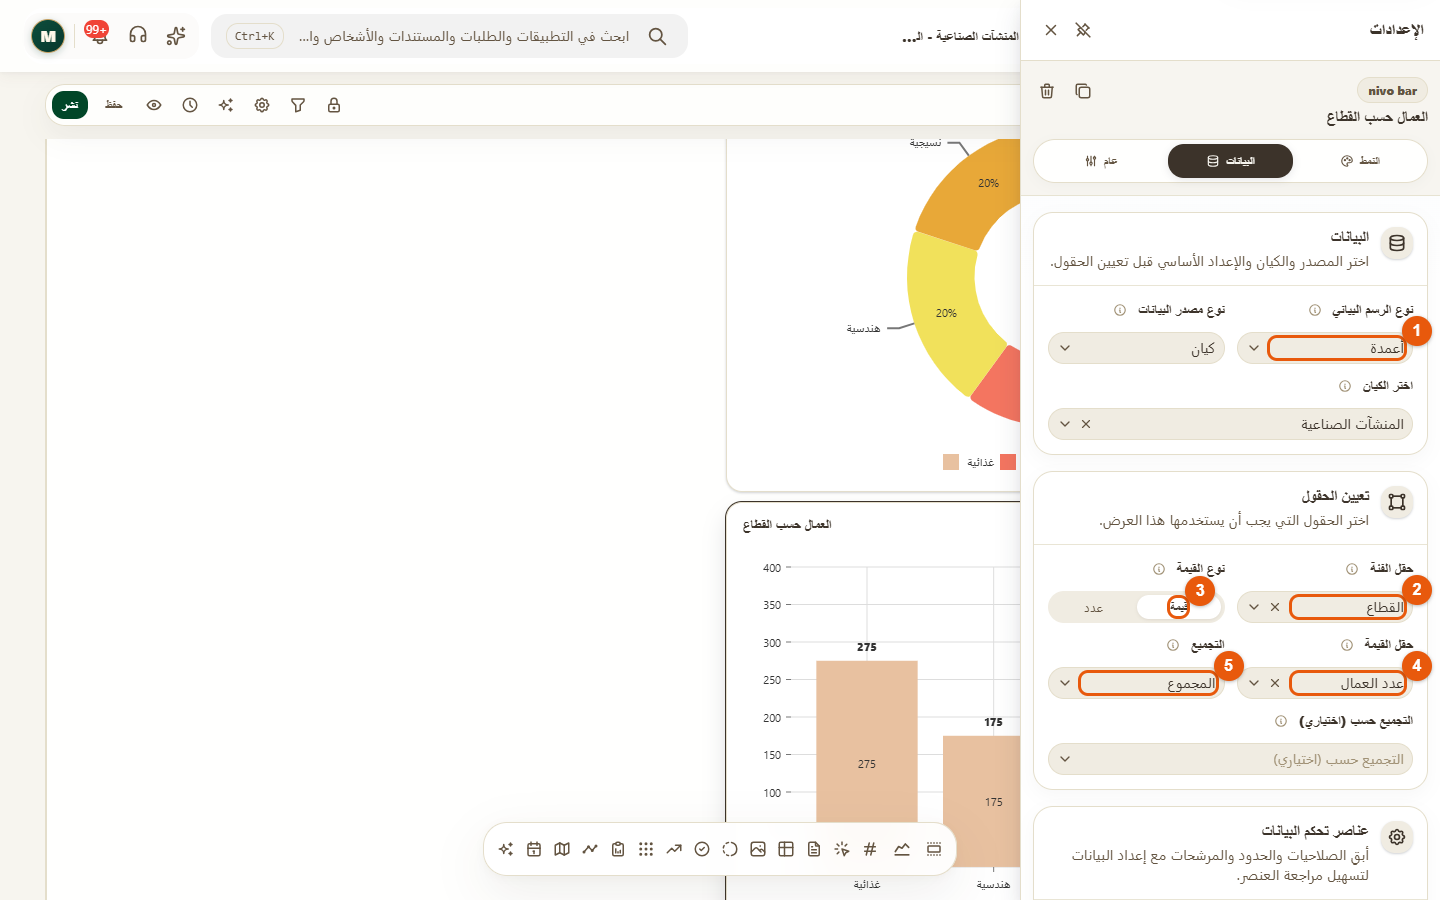
\includegraphics[width=0.95\linewidth]{assets/screens/i-bar.png}
\caption{ربط حقول رسم الأعمدة}
\label{fig:build-bar}
\shotnote{يرسم العنصر بيانات تجريبية حتى تختار «كيان»، ثم يرسم سجلاتك. ① «نوع الرسم البياني». ② «حقل الفئة»: ما يظهر تحت الأعمدة. ③ «نوع القيمة»: «عدد» أو «قيمة». ④ «حقل القيمة». ⑤ «التجميع».}
\end{figure}

\begin{figure}[H]
\centering
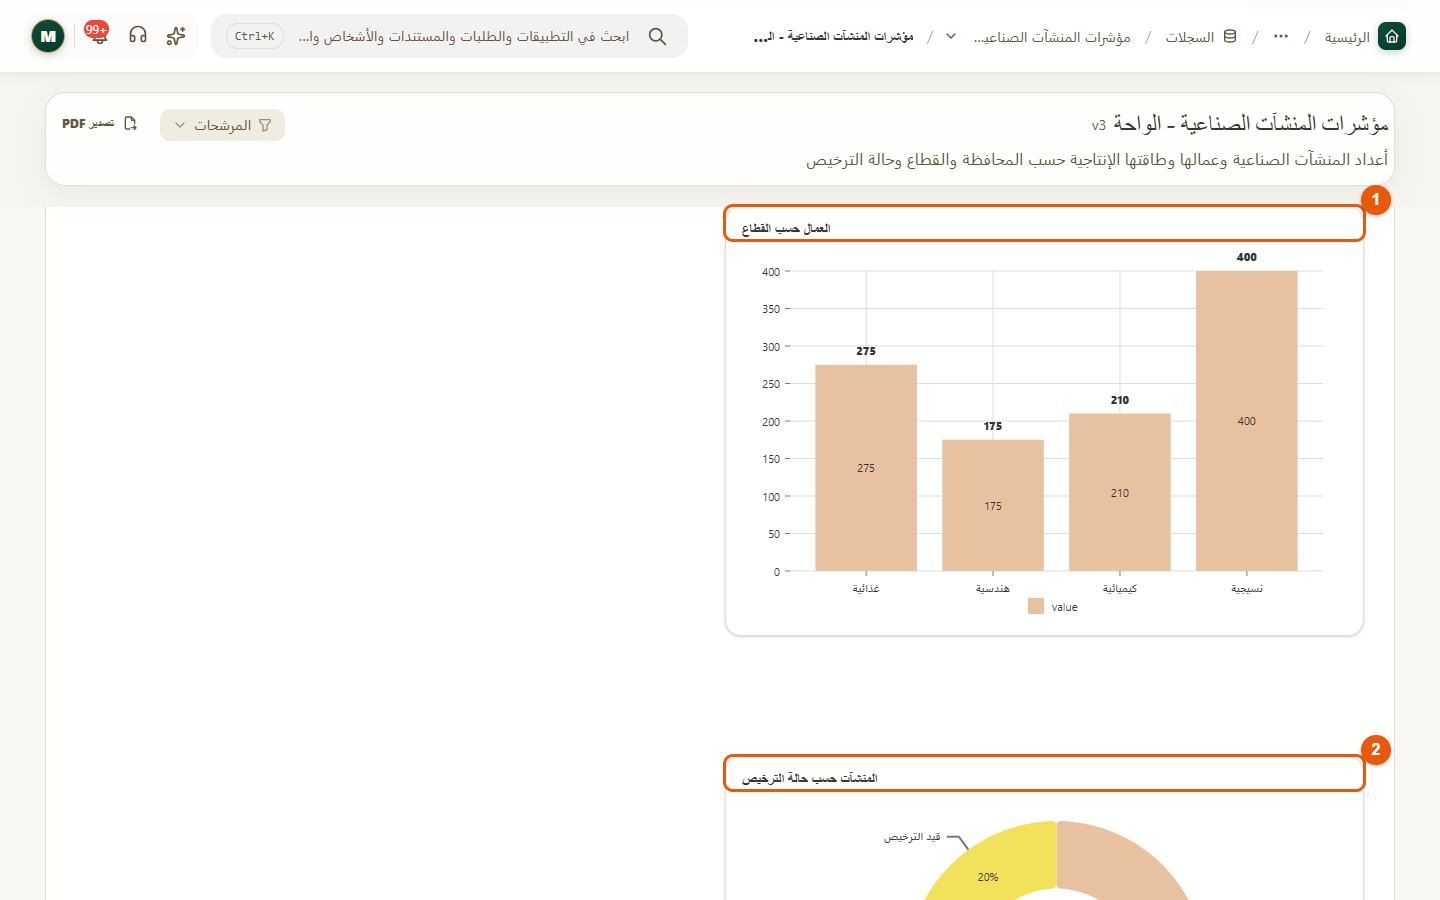
\includegraphics[width=0.95\linewidth]{assets/screens/i-view2.png}
\caption{الرسمان كما يراهما المشاهد}
\label{fig:build-charts-view}
\shotnote{يكتب الرسم القيمة فوق كل عمود، ويكتب الرسم الدائري النسبة على كل جزء. ① «العمال حسب القطاع». ② «المنشآت حسب حالة الترخيص».}
\end{figure}

\subsection{خطوات العمل والتحقق}
\begin{enumerate}
\item اضغط «إضافة رسم بياني (Nivo)»، واختر «أعمدة» أو «دائري».
\item في «البيانات» اختر «كيان»، ثم نوع السجلات، ثم «حقل الفئة».
\item للأعمدة اختر «نوع القيمة»: «عدد» للعدّ، أو «قيمة» ثم «حقل القيمة» ثم «التجميع». واختر الفئة أولاً؛ فتغييرها بعد ذلك يفرغ «حقل القيمة».
\item للجدول اضغط «جدول»، واختر «كيان» ونوع السجلات، ثم حدّد الأعمدة في «اختر الحقول».
\item سمِّ كل عنصر من «عام»، ثم اضغط «حفظ».
\end{enumerate}

\begin{figure}[H]
\centering
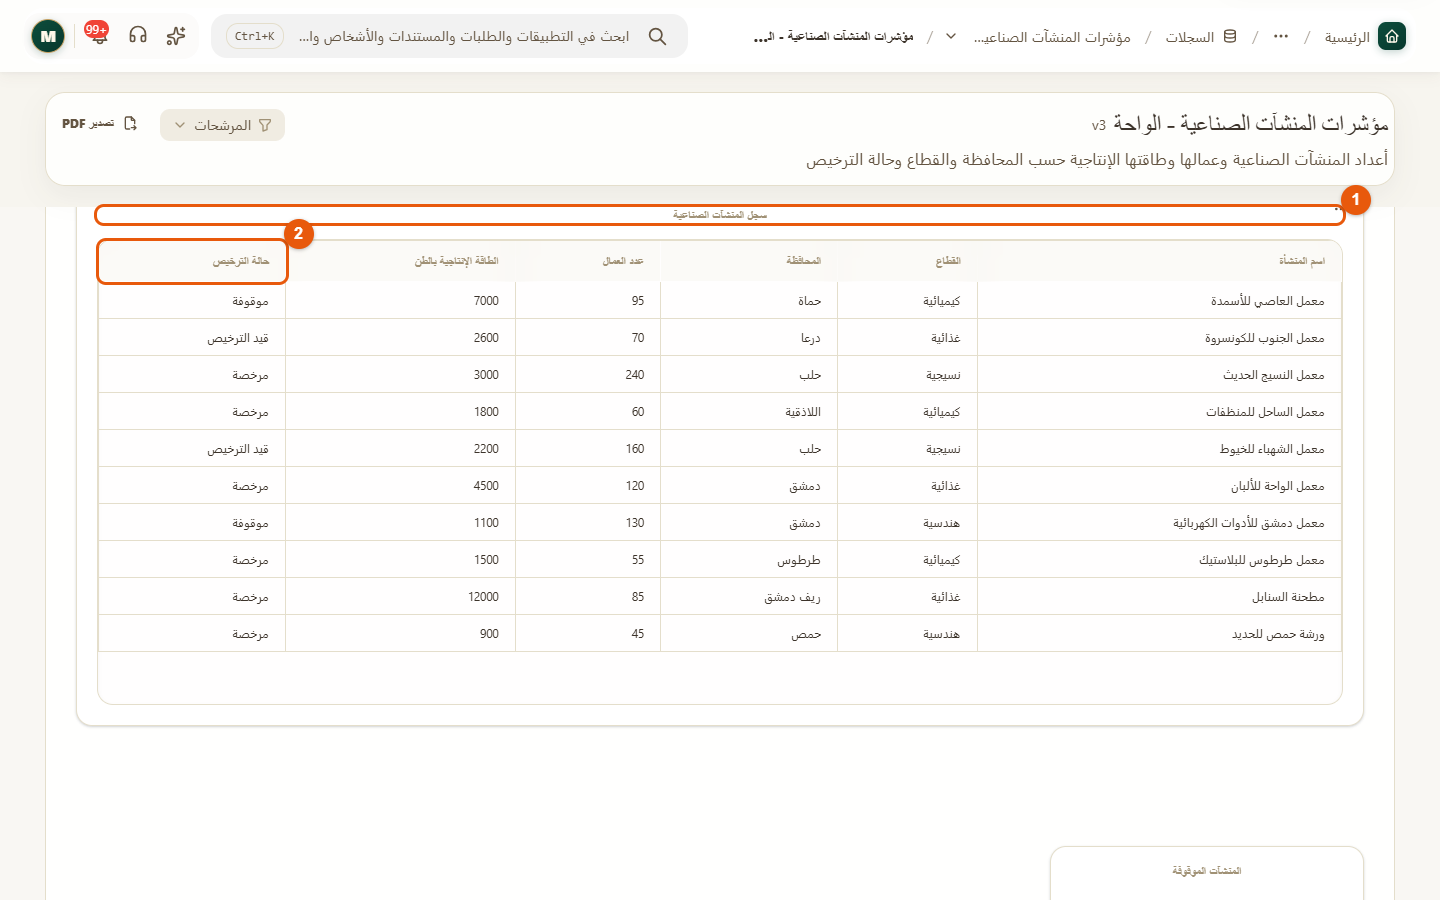
\includegraphics[width=0.95\linewidth]{assets/screens/i-view3.png}
\caption{جدول المنشآت}
\label{fig:build-table}
\shotnote{يعرض الجدول السجلات نفسها التي تُحسب منها الأرقام، فيستطيع المشاهد أن يتحقق منها. ① عنوان الجدول. ② عمود «حالة الترخيص».}
\end{figure}

\textbf{تحقق:} اجمع عمال القطاع الغذائي من القائمة يدوياً، ويجب أن يساوي العمود: 120 + 85 + 70 = 275.

\section{احسب عدداً بشرط}
\label{sec:build-widget-filter}

يحسب العنصر كل السجلات ما لم تضف إليه تصفية. والتصفية شرط ثابت داخل العنصر: «حيث» حقل «يساوي» قيمة. وقيمة حقل الاختيار هي مفتاحه المحفوظ لا نصه الظاهر، كما في القيم الافتراضية للنماذج.

\begin{rcnote}[مثال: مديرية الواحة]
مؤشر «المنشآت الموقوفة» يعدّ المنشآت حيث «حالة الترخيص» يساوي \en{mwqwft}، وهو مفتاح «موقوفة». فيعطي 2: معمل العاصي للأسمدة ومعمل دمشق للأدوات الكهربائية.
\end{rcnote}

\begin{figure}[H]
\centering
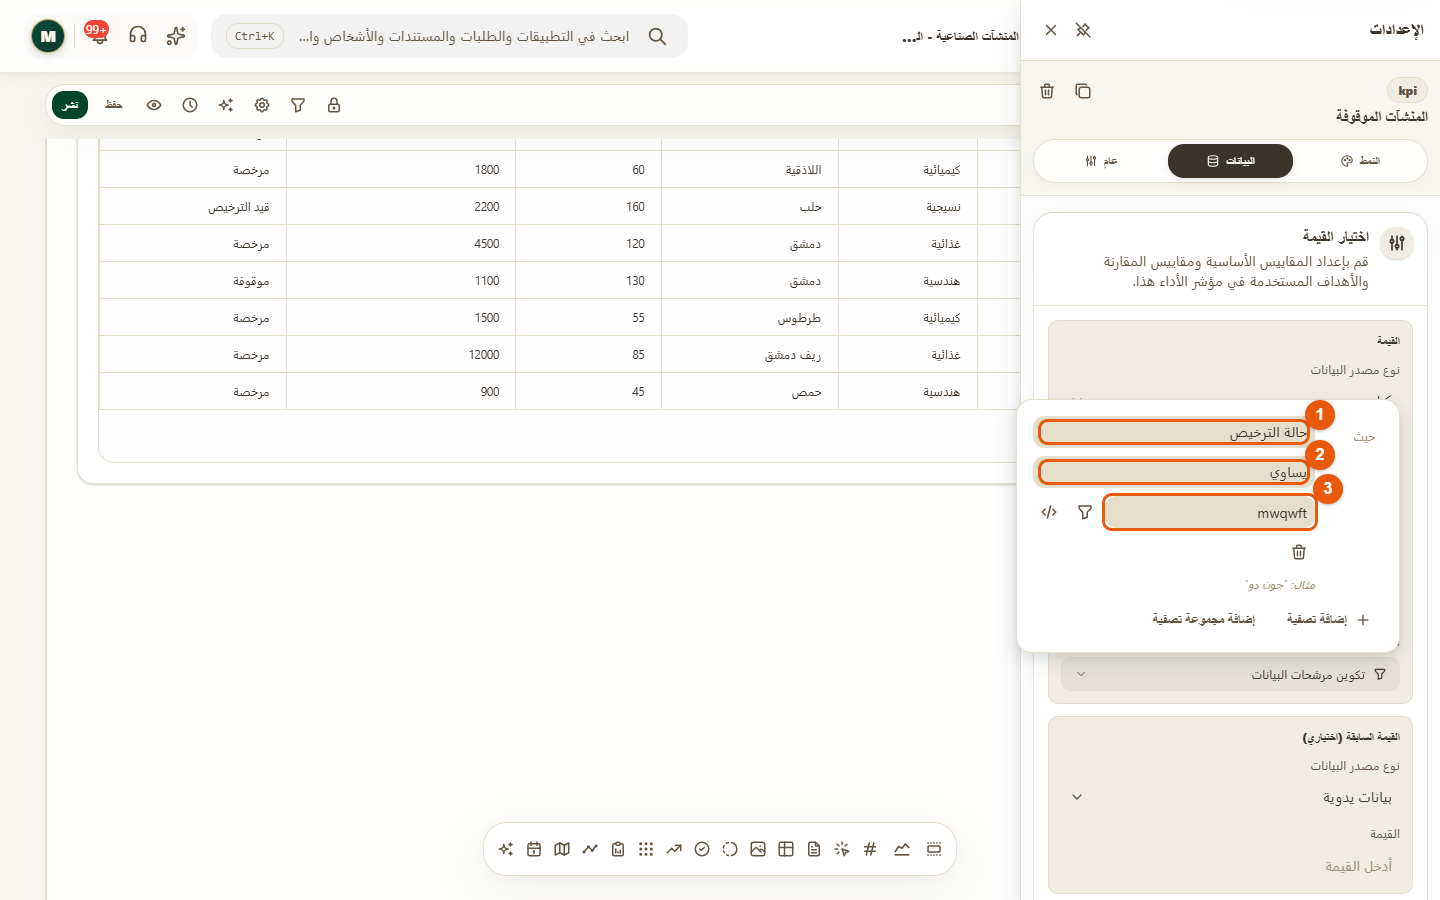
\includegraphics[width=0.95\linewidth]{assets/screens/i-wfilter.png}
\caption{تصفية داخل العنصر}
\label{fig:build-widget-filter}
\shotnote{يُكتب المفتاح كما هو بلا علامتي تنصيص، لأن الحقل قيمة لا تعبير. ① الحقل. ② «يساوي». ③ القيمة: مفتاح الخيار.}
\end{figure}

\subsection{خطوات العمل والتحقق}
\begin{enumerate}
\item اعرف مفتاح الخيار: افتح نوع السجلات ← «الحقول» ← الحقل، فيظهر المفتاح بجانب كل خيار في «الاختيارات».
\item في «البيانات» تحت «المرشحات»، اضغط «تكوين مرشحات البيانات» ← «إضافة تصفية».
\item اختر الحقل، واترك «يساوي»، واكتب المفتاح في «القيمة».
\end{enumerate}

\textbf{تحقق:} يجب أن يساوي الرقم عدد السجلات «موقوفة» في القائمة. وإذا ظهر 0، فقد كتبت النص بدل المفتاح.

\section{اربط اللوحة بالتطبيق وشاركها ثم انشر}
\label{sec:build-dashboard-publish}

لا تظهر اللوحة في التطبيق حتى تحدد مكانها، ولا يراها أحد حتى تشاركها وتنشرها. وتُحسب «بصلاحيات المشاهد»، لذلك يحتاج المشاهد أيضاً إلى «قائمة» و«فتح» على نوع السجلات، وإلا ظهرت له العناصر بلا بيانات.

\begin{rcnote}[مثال: مديرية الواحة]
وُضعت اللوحة في تطبيق «حماية المستهلك - الواحة» ← «السجلات»، وشوركت مع منصب «رئيس فريق الكشف» بصلاحية \en{Viewer}. ومُنح دور «رئيس فريق الواحة» «قائمة» و«فتح» على «المنشآت الصناعية»، ثم نُشرت.
\end{rcnote}

\begin{figure}[H]
\centering
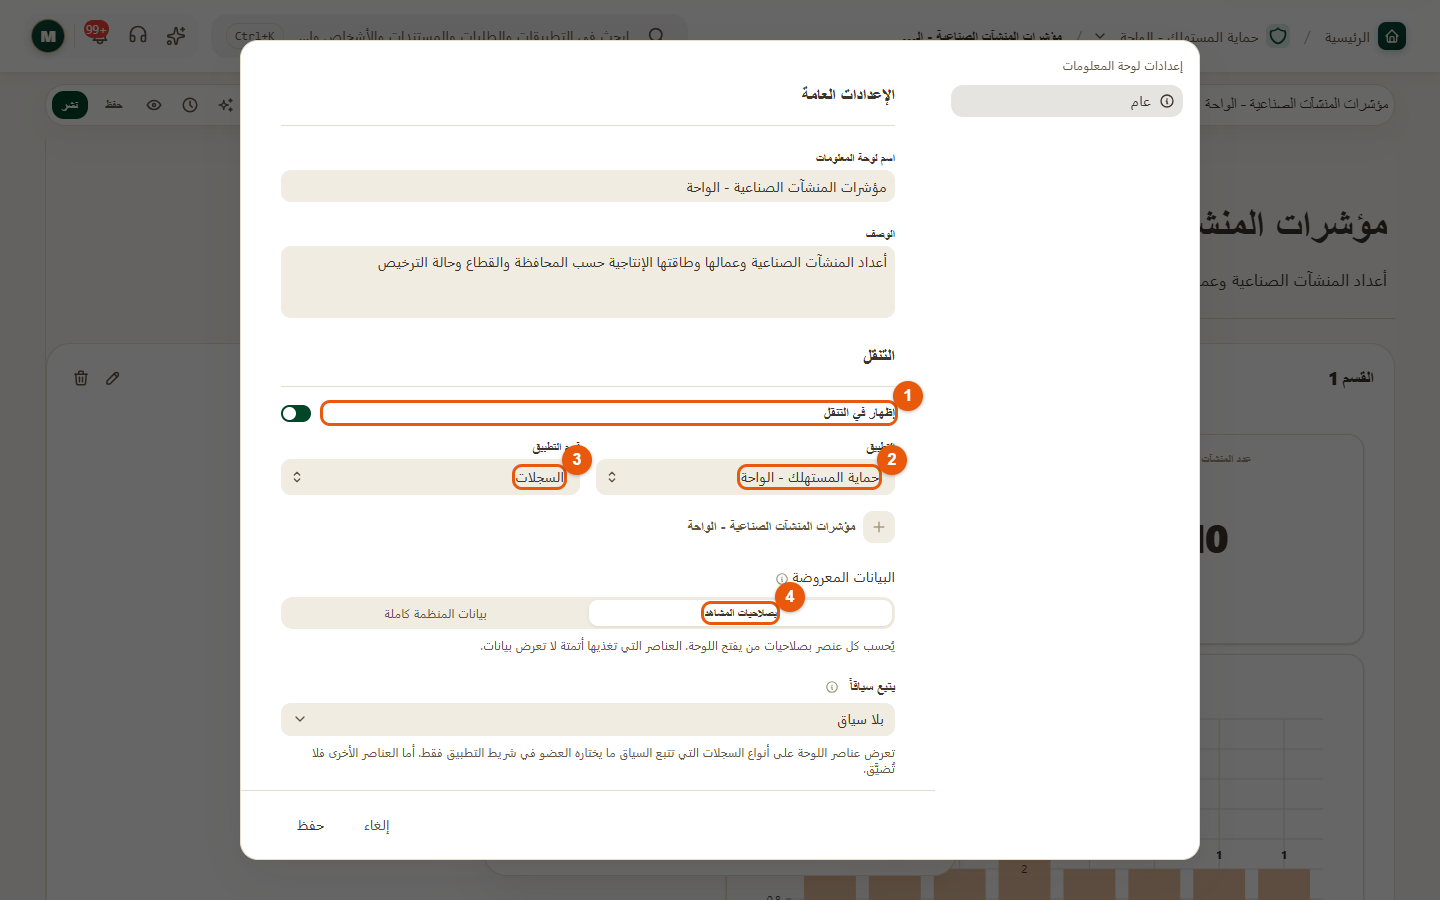
\includegraphics[width=0.95\linewidth]{assets/screens/i-settings.png}
\caption{مكان اللوحة في التطبيق}
\label{fig:build-dashboard-settings}
\shotnote{يظهر التطبيق والقسم بعد تفعيل الإظهار فقط، كما في نوع السجلات. ① «إظهار في التنقل». ② «التطبيق». ③ «قسم التطبيق». ④ «البيانات المعروضة»: «بصلاحيات المشاهد» يحسب كل عنصر بصلاحيات من يفتح اللوحة.}
\end{figure}

\begin{figure}[H]
\centering
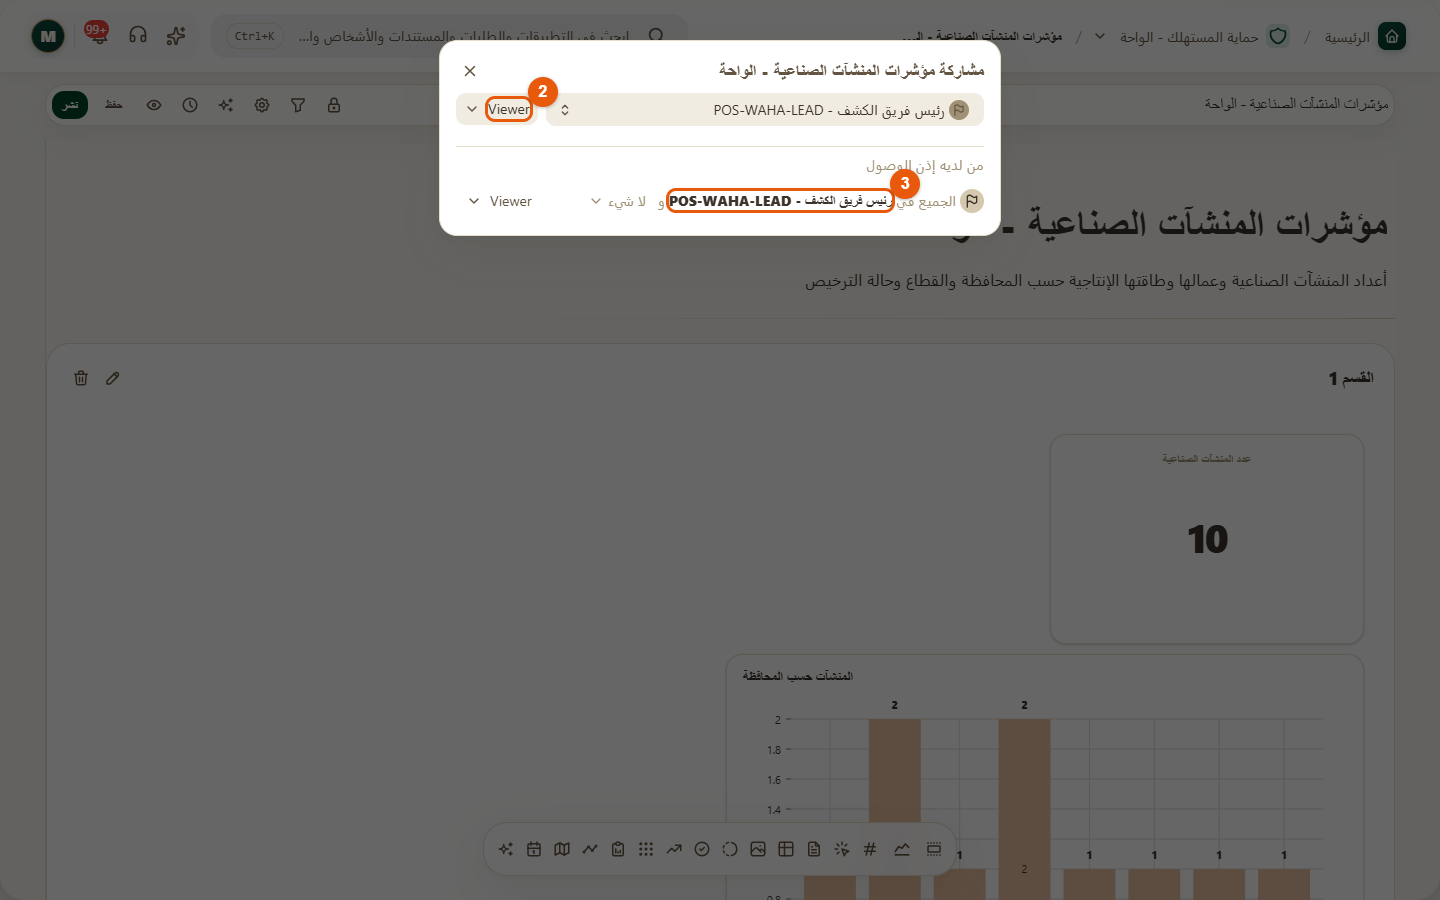
\includegraphics[width=0.62\linewidth]{assets/screens/i-share.png}
\caption{مشاركة اللوحة}
\label{fig:build-dashboard-share}
\shotnote{تُشارك اللوحة مع منصب أو عضو أو مجموعة، كما يُسند الدور. ① حقل الاختيار. ② مستوى الوصول: \en{Viewer} للمشاهدة فقط. ③ المنصب الذي شوركت معه.}
\end{figure}

\subsection{خطوات العمل والتحقق}
\begin{enumerate}
\item اضغط «الإعدادات»، وفعّل «إظهار في التنقل»، واختر «التطبيق» و«قسم التطبيق»، واترك «بصلاحيات المشاهد»، ثم اضغط «حفظ».
\item اضغط «إدارة الوصول»، وابحث عن المنصب واختره، واترك المستوى \en{Viewer}.
\item افتح نوع السجلات ← «الصلاحيات»، وامنح دور المشاهد «قائمة» و«فتح»، ثم «المراجعة والنشر» ← «نشر».
\item اضغط «نشر» في اللوحة.
\end{enumerate}

\textbf{تحقق:} ادخل بحساب المشاهد، وافتح التطبيق، ثم «لوحات المؤشرات». يجب أن تظهر اللوحة برقم الإصدار الجديد وبالأرقام نفسها.

\begin{figure}[H]
\centering
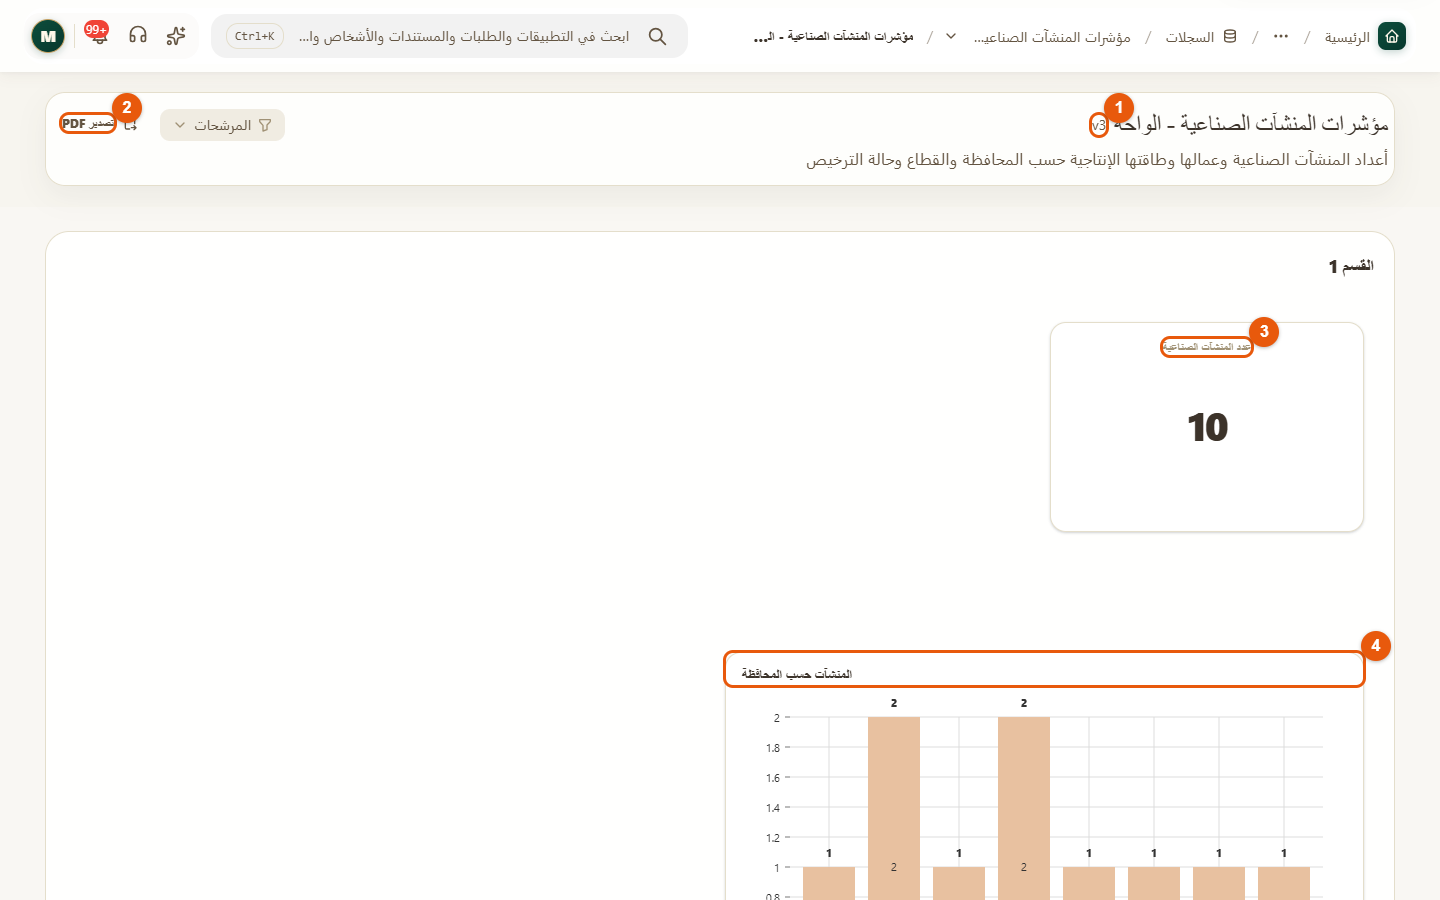
\includegraphics[width=0.95\linewidth]{assets/screens/i-view.png}
\caption{اللوحة بحساب رئيس الفريق}
\label{fig:build-dashboard-view}
\shotnote{هذه اللوحة كما يفتحها رئيس الفريق من التطبيق، وأرقامها مطابقة لما في المحرر. ① رقم الإصدار المنشور: إذا ظهر رقم قديم، فلم تُنشر آخر التعديلات. ② «تصدير PDF». ③ «عدد المنشآت الصناعية». ④ «المنشآت حسب المحافظة».}
\end{figure}

\section{مشكلات صادفناها وحلّها}
\label{sec:build-issues}

ظهرت هذه المشكلات أثناء التنفيذ الفعلي، وكلها سهلة الحل متى عُرف سببها. ويبيّن الجدول أين تظهر كل منها وكيف تُعالج.

\begin{rcnote}[مثال: مديرية الواحة]
اعتمدت رنا أول كشف ولم تتغير المنشأة. فتح مسؤول النظام «السجلات» في الكشف، فوجد السبب «قيم غير صالحة» في «حالة التوثيق»، فصحّح القيمة الافتراضية ونجح الكشف التالي.
\end{rcnote}

\begin{table}[H]
\centering
\caption{المشكلات وحلولها}
\label{tab:build-issues}
\begin{tabularx}{\linewidth}{R{5.2cm} Y}
\rcHeaderRow
\thh{ما ظهر} & \thh{السبب والحل}\\
«تمت الموافقة — تعذّر تطبيق التغييرات» و«قيم غير صالحة» & القيمة الافتراضية نص الخيار لا مفتاحه، أو «متكرر» مفعّل. اكتب المفتاح بين علامتي تنصيص، وأوقف «متكرر»، ثم انشر.\\
«بانتظار موافقة مسؤول» في لوحة «السجلات» & لم يُسمح للنموذج بالكتابة. اضغط «السماح في نوع السجل» ثم «موافقة».\\
النموذج غير متاح عند إنشاء الخطة & التكليف متوقف. اضغط «تشغيل التكليف»، أو فعّل «يمكن التكليف به» ثم انشر.\\
أزرار القرار معطلة عند المدقق & لم تُقرأ كل الأقسام، أو لم يُكتب التعليق المطلوب.\\
الصلاحيات لا تعمل & ما زالت مسودة. اضغط «المراجعة والنشر» في نوع السجلات.\\
النسخة الموقّعة بالإنجليزية & اللغة الافتراضية للمؤسسة الإنجليزية. اجعلها العربية من «إعدادات المؤسسة».\\
«خطأ: Invalid expression token» في القاعدة & النص في القيمة الافتراضية بلا علامتي تنصيص.\\
«ليس لديك صلاحية لعرض هذه البيانات» في عنصر & اخترت نوع سجلات آخر بالاسم نفسه، أو لا يملك المشاهد «قائمة» و«فتح» عليه.\\
عنصر بتصفية يعطي 0 & القيمة نص الخيار لا مفتاحه.\\
رسم أعمدة يعدّ بدل أن يجمع & «حقل القيمة» فارغ؛ فقد أفرغه تغيير «حقل الفئة». اختره من جديد.\\
المشاهد يرى إصداراً قديماً & لم تُنشر اللوحة بعد التعديل. اضغط «نشر».\\
مرشح المشاهد لا يغيّر الأرقام & مرشح «اختر الحقل» لا يُربط حالياً بحقل العناصر من الواجهة. استخدم التصفية داخل العنصر.\\
\end{tabularx}
\end{table}
